\part{B-Alberi vs Alberi Binari di Ricerca - Esercizio 1}

\begin{tcolorbox}[colback=lightgray!20,%gray background
                  colframe=black,% black frame colour
                  arc=3mm, auto outer arc,]
                  
    \textbf{Esercizio 1}
    \begin{itemize}
    
    \item Vogliamo analizzare le differenze tra B-Alberi e Alberi Binari di Ricerca

    \item I B-alberi (capitolo 18 libro di testo) sono strutture dati per memoria secondaria in cui ogni nodo può avere molti figli.

    \begin{itemize}
        \item Implementare B-alberi e confrontarli con la memorizzazione in alberi binari di ricerca
        \item in memoria secondaria gli algoritmi si confrontano sulla base degli accessi a disco (in questo caso possiamo considerare il numero di nodi letti o scritti)
    \end{itemize}
    
    \item Per fare questo dovremo:
    
        \begin{itemize}
          
            \item Scrivere i programmi Python (no notebook) che:
          
            \begin{itemize}
            
                \item implementino quanto richiesto
                
                \item eseguono un insieme di test che ci permettano di comprendere vantaggi e svantaggi delle diverse implementazioni
                
            \end{itemize}
                
            \item Svolgere ed analizzare opportuni esperimenti
            
            \item Scrivere una relazione (in LATEX) che descriva quanto fatto
            
        \end{itemize}
    \end{itemize}
    
\end{tcolorbox}

\section{Spiegazione teorica del problema - Esercizio 1}

\subsection{Introduzione}
\label{sec:Introduzione_1}
In questo parte del progetto si descrive l'implementazione degli alberi binari di ricerca e dei b-alberi e li mettiamo a confronto valutando la complessità computazionale di alcuni dei metodi che hanno logicamente in comune. Ci concentreremo, in particolare, sui metodi di inserimento e ricerca perché sono fondamentalmente i metodi più importanti e con ogni probabilità quelli maggiormente utilizzati quando si fa riferimento a degli alberi. Non confronteremo invece il metodo di cancellazione il quale è difficilmente implementabile nei b-alberi.

\subsection{Aspetti fondamentali}
\label{sec:AspettiFondamentali_1}
Nell'esperimento considereremo caso quello medio, ovvero una serie di numeri non ordinati, dunque in ordine casuale che vanno da n=step con $step=50$ a ```step*nTests```, con $nTests=20$, arriverà fino a $50*20=1000$. Dunque prenderemo la costruzione in modo casuale dell'albero (essenzialmente vuol dire che il numero che andrò ad inserire di volta in volta è casuale). Da qui in poi ci riferiremo agli Alberi Binari di Ricerca come ABR e ai B-Alberi come BA. Useremo anche alcune parti fondamentali della nomenclatura della teoria della complessità computazionale come $O(\cdot)$ e $\Theta(\cdot)$. Ci riferiremo anche ad $n$ come numero di nodi dell'albero ed ad $h = \log _t n$ come altezza dell'albero. Non utilizzeremo altre strutture dati particolari all'infuori degli alberi in questione. Descriviamo brevemente i metodi che andremo ad analizzare in particolare:
\begin{itemize}
    \item Inserimento
    \begin{itemize}
        \item ABR: 
        \begin{enumerate}
            \item Inizio:\\
                L'inserimento inizia dalla radice dell'albero.
            \item Ricerca della Posizione:\\
                Si procede verso il basso confrontando la chiave da inserire con le chiavi nei nodi dell'albero.\\
                Se la chiave da inserire è minore della chiave del nodo corrente, si continua la ricerca nel sottoalbero sinistro.\\
                Se invece la chiave è maggiore, si continua la ricerca nel sottoalbero destro.
            \item Inserimento:\\
                La chiave da inserire viene posizionata in un nuovo nodo nel punto in cui termina la ricerca, in un nodo vuoto o sostituendo un nodo esistente.\\
                Se il nodo di destinazione ha già un figlio a sinistra o a destra, la chiave viene inserita come figlio sinistro o destro, mantenendo l'ordinamento del ABR.
            \item Fine:
                L'inserimento è completato e non c'è nessun ribilanciamento dell'albero.
        \end{enumerate}
    
        \item BA:
        \begin{enumerate}
            \item Inizio:\\
                L'inserimento inizia nella radice dell'albero.
            \item Ricerca del Nodo Adeguato:\\
                Inizia la ricerca del nodo appropriato per l'inserimento. Si discende nell'albero seguendo i rami in base ai valori chiave fino a raggiungere una foglia o un nodo interno.
            \item Inserimento nel Nodo:\\
                Se il nodo in cui ci troviamo non è completamente pieno, possiamo semplicemente inserire la nuova chiave nel nodo mantenendo l'ordinamento.\\
                Se il nodo è pieno, viene diviso in due nodi più piccoli. La chiave mediana viene promossa al genitore e i due nuovi nodi contengono le chiavi rimanenti divise in modo equo.
            \item Propagazione delle Promozioni:\\
                Se la promozione raggiunge la radice, la radice viene divisa generando un nuovo livello nell'albero.
            \item Aggiornamento dei Puntatori:\\
                Durante l'inserimento e la divisione, i puntatori dei nodi vengono aggiornati per riflettere la nuova struttura dell'albero.
            \item Fine:\\
                L'inserimento è completato e c'è ribilanciamento dell'albero ad ogni elemento inserito.
        \end{enumerate}
    \end{itemize}
    
    \item Ricerca
    \begin{itemize}
        \item ABR: 
        \begin{enumerate}
            \item Inizio:\\
                La ricerca inizia dalla radice dell'albero.
            \item Confronto con il Nodo Corrente:\\
                Si confronta la chiave da cercare con la chiave del nodo corrente.\\
                Se la chiave corrisponde, la ricerca è terminata e il nodo è stato trovato.\\
                Se la chiave è minore della chiave del nodo corrente, si sposta nel sottoalbero sinistro (poiché tutte le chiavi nel sottoalbero sinistro sono minori di quella del nodo corrente).\\
                Se la chiave è maggiore, si sposta nel sottoalbero destro (poiché tutte le chiavi nel sottoalbero destro sono maggiori di quella del nodo corrente).
            \item Ricerca Ricorsiva:\\
                Il passo 2 è ripetuto in modo ricorsivo nel sottoalbero scelto.\\
                Questo processo continua fino a quando viene trovato il nodo con la chiave cercata o si raggiunge una foglia dell'albero senza trovare la chiave.
            \item Fine:\\
                La ricerca termina quando viene trovato il nodo con la chiave cercata o quando si raggiunge una foglia senza trovare la chiave cercata.
        \end{enumerate}        
        \item BA: 
        \begin{enumerate}
            \item Inizio:\\
                La ricerca inizia dalla radice dell'albero.
            \item Confronto con le Chiavi:\\
                Si confronta la chiave da cercare con le chiavi presenti nel nodo corrente.\\
                Se la chiave è presente nel nodo, la ricerca è terminata, e viene restituito il valore associato alla chiave.\\
                Se la chiave è minore della chiave minima nel nodo, si scende nel sottoalbero sinistro.\\
                Se la chiave è maggiore della chiave massima nel nodo, si scende nel sottoalbero destro.\\
                Se la chiave è compresa tra le chiavi minima e massima, si scende nel sottoalbero corrispondente.
            \item Ricerca Ricorsiva:
                Il passo 2 viene ripetuto in modo ricorsivo nel sottoalbero selezionato.\\
                Questo processo continua fino a quando viene trovata la chiave nel nodo o si raggiunge una foglia dell'albero senza trovare la chiave cercata.
            \item Fine:\\
                La ricerca termina quando viene trovato il nodo con la chiave cercata o quando si raggiunge una foglia senza trovare la chiave cercata.
        \end{enumerate}
    \end{itemize}
\end{itemize}
Ora vorrei descrivere le particolarità di queste due tipologia di alberi partendo da ABR. 
Le proprietà di un ABR (esempio in figura \ref{fig:ABR}) sono:
\begin{enumerate}
    \item Il sottoalbero sinistro di un nodo $x$ contiene soltanto i nodi con chiavi minori della chiave del nodo $x$.
    \item Il sottoalbero destro di un nodo $x$ contiene soltanto i nodi con chiavi maggiori della chiave del nodo $x$.
    \item Il sottoalbero destro e il sottoalbero sinistro devono essere entrambi due ABR.
\end{enumerate}
Le proprietà di un BA (esempio in figura \ref{fig:BA}) sono:
\begin{enumerate}
    \item Ogni nodo $x$ ha i seguenti attributi:
    \begin{itemize}
        \item $x.n$ è il numero di chiavi correttamente memorizzate nel nodo $x$.
        \item Le $x.n$ chiavi stesse, $x.key_1,...,x.key_x_._n$ sono memorizzate in ordine non decrescente, in modo che: \(x.key_1\leq x.key_2\leq ...\leq x.key_x_._n\).
        \item $x.leaf$ è un valore booleano che è TRUE se $x$ è una foglia, e invece è FALSE se $x$ è un nodo interno.
    \end{itemize}
    \item Ogni nodo interno $x$ contiene anche $x.n+1$ puntatori $x.c_1 ,...,x.c_x_._n_+_1$ ai suoi figli. I nodi foglia non hanno figli, quindi i loro attributi $c_i$ non sono definiti.
    \item Le chiavi $x.key_i$ separano gli intervalli delle chiavi memorizzate in ciascun sottoalbero: se $k_i$ è una chiave qualsiasi memorizzata nel sottoalbero con radice $c_i[x]$ allora:\\
    \(k_1\leq x.key_1\leq k_2\leq x.key_2\leq ...\leq x.key_x_._n\leq x.key_x_._n_+_1\)
    \item Tutte le foglie hanno la stessa profondità, che è l'altezza $h$ dell'albero.
    \item Ci sono limiti superiori e inferiori al numero di chiavi che un nodo può contenere. Questi limiti possono essere espressi in termini di un intero \(t\geq2\) chiamato \textbf{grado minimo} del BA:
    \begin{itemize}
        \item Ogni nodo, tranne la radice deve avere almeno $t-1$ chiavi- Ogni nodo interno, tranne la radice, quindi almeno $t$ figli. Se l'albero non è vuoto la radice deve avere almeno una chiave.
        \item Ogni nodo può contenere al massimo $2t-1$ chiavi. Quindi un nodo interno può avere al massimo $2t$ figli. Diciamo che un nodo è \textbf{pieno} se contiene esattamente $2t-1$ chiavi.
    \end{itemize}
\end{enumerate}

\begin{figure}[H]
    \centering
    \begin{subfigure}[H]{0.35\textwidth}
        \centering
        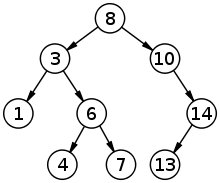
\includegraphics[width=1\textwidth]{Images/ABR.png}
        \caption{Albero binario di ricerca}
        \label{fig:ABR}
    \end{subfigure}
    \hfill
    \begin{subfigure}[H]{0.6\textwidth}
        \centering
        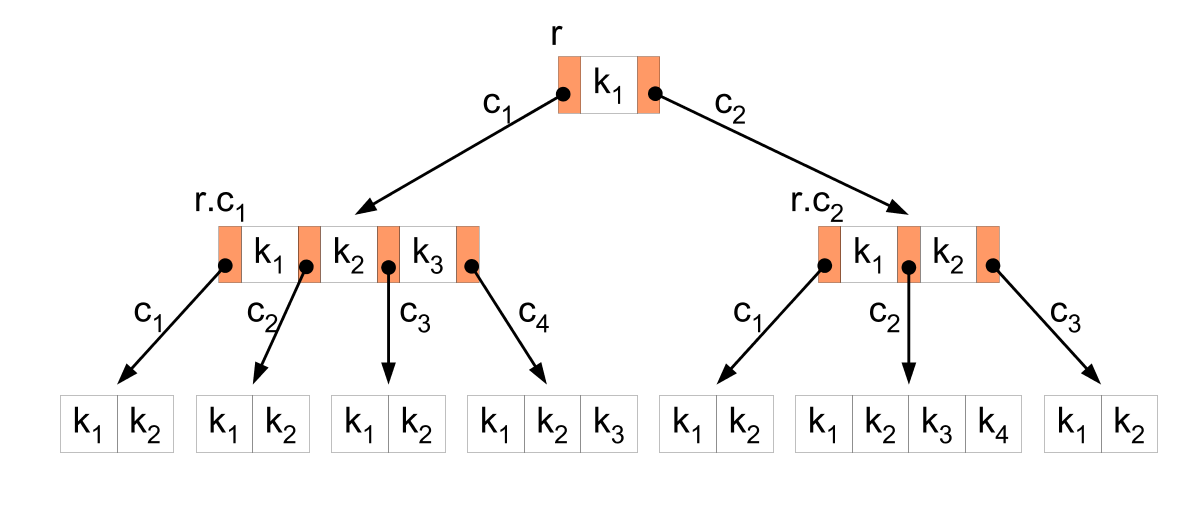
\includegraphics[width=1\textwidth]{Images/BA.png}
        \caption{B-Albero}
        \label{fig:BA}
    \end{subfigure}
    \caption{Tipologie di alberi}
\end{figure}

\subsection{Assunti ed ipotesi}
\label{sec:AssuntiEdIpotesi_1}
In un ABR le operazioni di base richiedono un tempo proporzionale all'altezza dell'albero. L'altezza attesa di un ABR costruito in modo casuale è $O(h)$ quindi le operazioni elementari svolte su questo tipo di albero richiedono in media $\Theta(h)$. Per vedere la complessità degli algoritmi più importanti di ABR basati sul caso peggiore e sul caso medio si richiama alla figura \ref{fig:ComplessitàABR} facendo particolare attenzione ai metodi in rosso che sono quelli su cui andremo a svolgere gli esperimenti.

\begin{figure}[H]
    \centering
    \begin{tabular}{|c|c|c|}
        \hline
         & Complessità al caso peggiore & Complessità al caso medio\\
        \hline
        Spazio & $\Theta$($n$) & $\Theta$($n$)\\
        \hline
        \textcolor{red}{Inserimento} & $O(n)$ & $O(h)$\\
        \hline
        \textcolor{red}{Ricerca} & $O(n)$ & $O(h)$\\
        \hline
        Cancellazione & $O(n)$ & $O(h)$\\
        \hline
    \end{tabular}
    \caption{Complessità degli algoritmi di ABR}
    \label{fig:ComplessitàABR}
\end{figure}

Per un B-albero, le operazioni di base richiedono un tempo proporzionale all'altezza dell'albero. La struttura di un B-albero permette di mantenere un bilanciamento dell'altezza e di ridurre la complessità delle operazioni rispetto a un albero binario di ricerca. Le operazioni di base su un B-albero richiedono in media \(\Theta(\log_t n)\), dove \(log_tn=h\) è l'altezza dell'albero e \(n\) è il numero di chiavi nell'albero. Qui di seguito sono presentate le complessità degli algoritmi più importanti di un B-albero, sia nel caso peggiore che nel caso medio.

\begin{figure}[H]
    \centering
    \begin{tabular}{|c|c|c|}
        \hline
         & Complessità al caso peggiore & Complessità al caso medio\\
        \hline
        Spazio & \(\Theta(n)\) & \(\Theta(n)\)\\
        \hline
        \textcolor{red}{Inserimento} & \(O(\log n)\) & \(O(\log n)\)\\
        \hline
        \textcolor{red}{Ricerca} & \(O(\log n)\) & \(O(\log n)\)\\
        \hline
        Cancellazione & \(O(\log n)\) & \(O(\log n)\)\\
        \hline
    \end{tabular}
    \caption{Complessità degli algoritmi di B-albero}
    \label{fig:ComplessitàBA}
\end{figure}


Il nostro obiettivo in questo test è verificare sperimentalmente la veridicità delle varie complessità descritte nelle figure \ref{fig:ComplessitàABR} e \ref{fig:ComplessitàBA} e capire sotto quali condizioni un albero è più conveniente di un altro confrontandoli, a parità di spazio, in base al tempo reale che ci mettono a completarsi.





\newpage
\section{Documentazione del codice - Esercizio 1}

\subsection{Scelte implementative}
\label{sec:ScelteImplementative_1}
Con la seguente descrizione elencheremo i vari attributi delle classi che permettono l'implementazione degli alberi binari di ricerca e dei b-alberi.

\begin{itemize}
    \item nessun padre
    \item colore nero
    \item chiave -1
\end{itemize}

\item \textbf{BinaryTreeNode}
    \begin{itemize}
        \item \textbf{key} : contiene il valore del nodo.
        \item \textbf{left} : è un puntatore al figlio sinistro.
        \item \textbf{right} : è un puntatore al figlio destro.
        \item \textbf{p} : è un puntatore al padre sinistro.
    \end{itemize}

\item \textbf{BinaryTree}
    \begin{itemize}
        \item \textbf{node} : contiene nodo.
        \item \textbf{root} : è un puntatore alla radice.
        \item \textbf{node\textunderscore read} : contarore che tiene nota di quante letture vengono fatte sull'albero.
        \item \textbf{node\textunderscore written} : contarore che tiene nota di quante scritture vengono fatte sull'albero.
    \end{itemize}

\item \textbf{BTreeNode}
    \begin{itemize}
        \item \textbf{leaf} : booleano vero se il nodo è una foglia.
        \item \textbf{keys} : lista con valori nel nodo.
        \item \textbf{child} : lista con puntatori ai figli.
        \item \textbf{n} : numero chiavi memorizzate nel nodo.
    \end{itemize}

\item \textbf{BTree}
    \begin{itemize}
        \item \textbf{root} : è un puntatore alla radice\textit{p}.
        \item \textbf{t} : numero minimo chiavi memorizzate in ogni nodo \textit{p}.
        \item \textbf{node\textunderscore read} : contarore che tiene nota di quante letture vengono fatte sull'albero \textit{p}.
        \item \textbf{node\textunderscore written} : contarore che tiene nota di quante scritture vengono fatte sull'albero\textit{p}.
    \end{itemize}

\subsection{Descrizione dei metodi implementati}
\label{sec:DescrizioneMetodiImplementati_1}
In questa parte descriverò le funzionalità di ogni metodo delle classi degli alberi.

\begin{itemize}

    \item \textbf{BinaryTree}
    \begin{itemize}

        \item \textbf{get\textunderscore node\textunderscore read()} : restituisce il numero di letture eseguite sull'albero.

        \item \textbf{get\textunderscore node\textunderscore written()} : restituisce il numero di scritture eseguite sull'albero.

        \item \textbf{search(x, key)} : in modo ricorsivo visita e quando trova una chiave ==key, ritorna quel nodo.
        
        \item \textbf{insert(key)} : in modo iterativo va avanti nell'albero fino a ricercare la foglia più vicina a key e se è maggiore inserisce a destra, e se minore a sinistra
        
    \end{itemize}
    
    \item \textbf{BinaryTree}
    \begin{itemize}

        \item \textbf{get\textunderscore node\textunderscore read()} : restituisce il numero di letture eseguite sull'albero.

        \item \textbf{get\textunderscore node\textunderscore written()} : restituisce il numero di scritture eseguite sull'albero.

        \item \textbf{search(key)} : in modo ricorsivo visita e quando trova una chiave == key, ritorna quel nodo e la sua profondità.

        \item \textbf{split\textunderscore child(x, i)} : divide un nodo figlio troppo grande in due nodi più piccoli durante un'operazione di inserimento. 
        
        \item \textbf{insert(key)} : inserisce la  chiave e usando \textbf{split child(x, i)} e \textbf{insert nonfull(key)} mantiene l'albero bilanciato.
        
        \item \textbf{insert\textunderscore nonfull(key)} : viene chiamata quando si inserisce una chiave in un nodo non completamente pieno.
        
    \end{itemize}
    
    \item \textbf{Generazione dei grafici}
    \begin{itemize}
    
        \item \textbf{random\textunderscore array(n)} : restituisce un'array ordinato casualmente con n valori da 1 a n.
        
        \item \textbf{test\textunderscore insert(BinaryTree, BTree, array)} : restituisce più valori contenenti i tempi di esecuzione in serie del metodo \textbf{insert} per ABR e BA, e delle rispettive occorrenze di lettura e scrittura. 
        
        \item \textbf{test\textunderscore search(BinaryTree, BTree, array)} : restituisce più valori contenenti i tempi di esecuzione in serie del metodo \textbf{search} per ABR e BA, e delle rispettive occorrenze di lettura e scrittura.
        
        \item \textbf{draw\textunderscore table(data, title, colorHead="orange", colorCell="yellow", filename="table")} : genera una tabella con la tupla data, e come stile della tabella prende i parametri in ingresso, e salva il tutto in memoria con il nome filename.
        
        \item \textbf{draw\textunderscore side\textunderscore graphs(left data, right data, plot title, filename)} : genera due grafici l'uno accanto all'altro, e salva il tutto in memoria con il nome filename.
        
        \item \textbf{draw\textunderscore comparison\textunderscore graphs(data1, data2, title, filename)} : genera grafico con entrambi i data nello stesso subplot, e salva il tutto in memoria con il nome filename.
        
    \end{itemize}
    
\end{itemize}

\newpage
\section{Descrizione degli esperimenti condotti e analisi dei risultati sperimentali - Esercizio 1}

\subsection{Dati utilizzati}
\label{sec:DatiUtilizzati_1}
L'esperimento che ho svolto si divide prima di tutto per il numero di nodi che sono andato ad inserire nei due alberi. Quindi divideremo l'esperimento in 4 parti:

\begin{itemize}
    \item Alberi con $t=\textbf{100}$
    \item Alberi con $t=\textbf{250}$
    \item Alberi con $t=\textbf{1000}$
\end{itemize}

Prendendo il caso della randomizzazione ho deciso di fare un test per verificare se il range in cui prendo i numeri influenzi il tempo che ci mette per lo svolgimento dell'algoritmo. Questo caso è stato testato con gli alberi da 1000 elementi per avere una miglior idea delle tempistiche. I range di valori che ho usato sono i seguenti:

\textbf{50-1000, con uno step di 50}
Quindi ho creato 20 array su cui testare il tutto, al variare della $\textbf{t}$

\subsection{Misurazioni}
\label{sec:Misurazioni_1}
I metodi di calcolo dei tempi nei metodi \textbf{test\textunderscore insert} e \textbf{test\textunderscore search} sono di due tipi. Innanzitutto dobbiamo prendere il tempo prima dell'esecuzione del metodo e quello dopo la sua esecuzione:

\begin{verbatim}
def test_search(BinaryTree, BTree, array):
    print(f"\nRicerca di {len(array)} elementi:")

    timesBin = 0
    timesBT = 0
    for i in range(len(array)):
        start = timer()
        BinaryTree.search(BinaryTree.root, array[i])
        end = timer()
        timesBin += (end - start) * 1000

        start = timer()
        BTree.search(array[i])
        end = timer()
        timesBT += (end - start) * 1000

    readBin = BinaryTree.get_node_read()
    writtenBin = BinaryTree.get_node_written()
    readBT = BTree.get_node_read()
    writtenBT = BTree.get_node_written()

    print(f"Albero binario di ricerca: {timesBin} ms")
    print(f"B-albero: {timesBT} ms")
    print(f"Albero binario di ricerca: {readBin} letture, {writtenBin} scritture")
    print(f"B-albero: {readBT} letture, {writtenBT} scritture")

    return timesBin, timesBT, readBin, readBT, writtenBin, writtenBT

def test_insert(BinaryTree, BTree, array):
    print(f"\nInserimento di {len(array)} elementi:")
    timesBin = 0
    timesBT = 0
    for i in range(len(array)):
        start = timer()
        BinaryTree.insert(BinaryTreeNode(array[i]))
        end = timer()
        timesBin += (end - start) * 1000

        start = timer()
        BTree.insert(array[i])
        end = timer()
        timesBT += (end - start) * 1000

    readBin = BinaryTree.get_node_read()
    writtenBin = BinaryTree.get_node_written()
    readBT = BTree.get_node_read()
    writtenBT = BTree.get_node_written()

    print(f"Albero binario di ricerca: {timesBin} ms")
    print(f"B-albero: {timesBT} ms")
    print(f"Albero binario di ricerca: {readBin} letture, {writtenBin} scritture")
    print(f"B-albero: {readBT} letture, {writtenBT} scritture")

    return timesBin, timesBT, readBin, readBT, writtenBin, writtenBT
\end{verbatim}

Per calcolare i tempi salvo in \textbf{start} il tempo prima dell'operazione, e in \textbf{end}. La loro sottrazione mi darà il tempo trascorso in nanosecondi, che moltiplicherò per 1000 per ottenerlo in millisecondi.     

\newpage
\subsection{Risultati sperimentali e commenti analitici}
\label{sec:RisultatiSperimentaliCommentiAnalitici_1}

Guardo prima i tempi di esecuzione:

\subsubsection{Alberi a confronto nei tempi con $t = 100$}
\begin{comment}
\begin{figure}[H]
    \centering
    \begin{subfigure}[b]{0.49\textwidth}
        \centering
        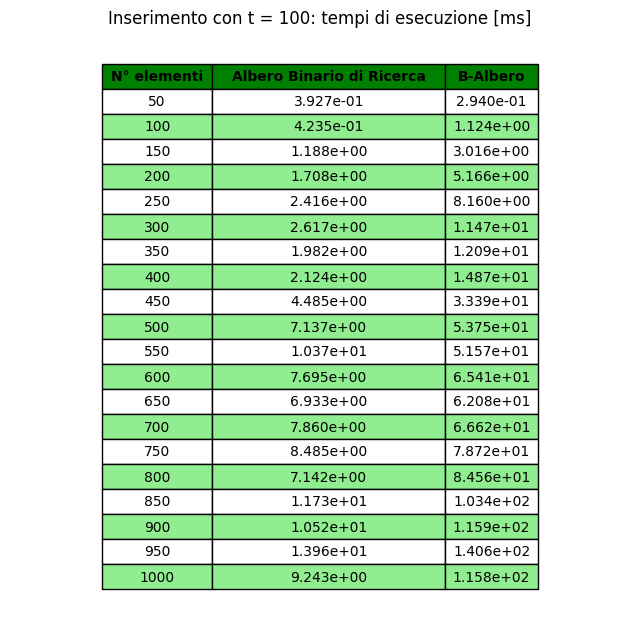
\includegraphics[width=\textwidth]{tables/insert-ms-t100.png}
        \caption{Inserimento}
        \label{fig:tableinserttimet100}
    \end{subfigure}
    \hfill
    \begin{subfigure}[b]{0.49\textwidth}
        \centering
        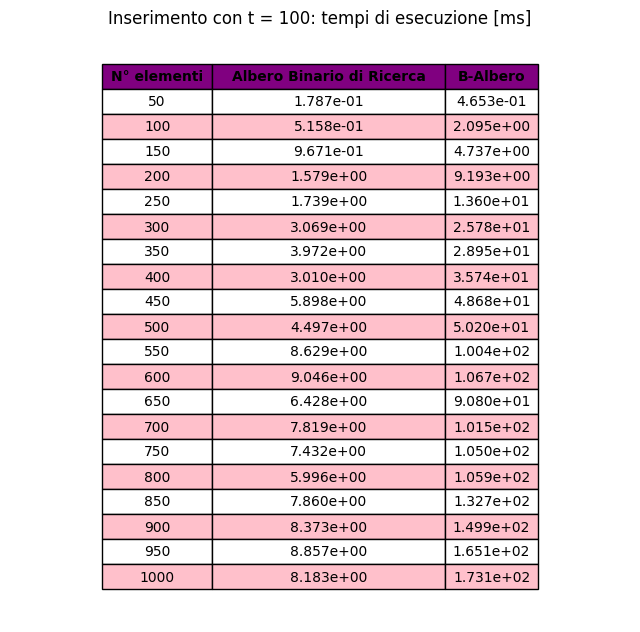
\includegraphics[width=\textwidth]{tables/search-ms-t100.png}
        \caption{Ricerca}
        \label{fig:tablesearchtimet100}
    \end{subfigure}
    \caption{Tabella tempi con $t=100$}
    \label{fig:tabletimest100}
\end{figure}
\end{comment}

\begin{figure}[H]
    \centering
    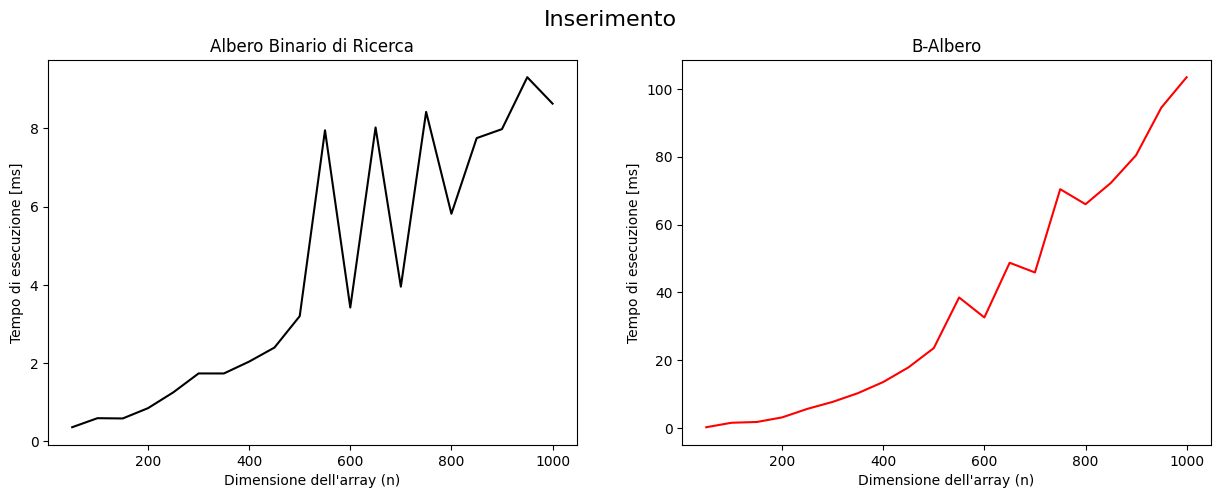
\includegraphics[width=\textwidth]{side-graphs/insert-ms-t100.png}
    \caption{Grafico tempi dell'Inserimento con $t=100$}
        \label{fig:sidegraphinserttimet100}
\end{figure}
    
\begin{figure}[H]
    \centering
    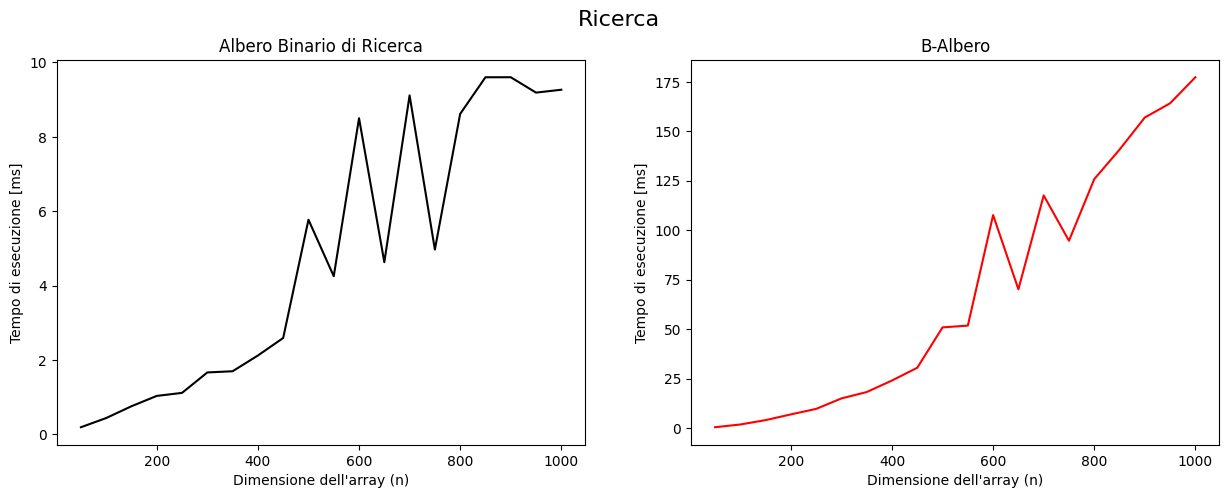
\includegraphics[width=\textwidth]{side-graphs/search-ms-t100.png}
    \caption{Grafico tempi della Ricerca con $t=100$}    \label{fig:sidegraphsearchtimet100}
\end{figure}

\begin{figure}[H]
    \centering
    \begin{subfigure}[b]{0.49\textwidth}
        \centering
        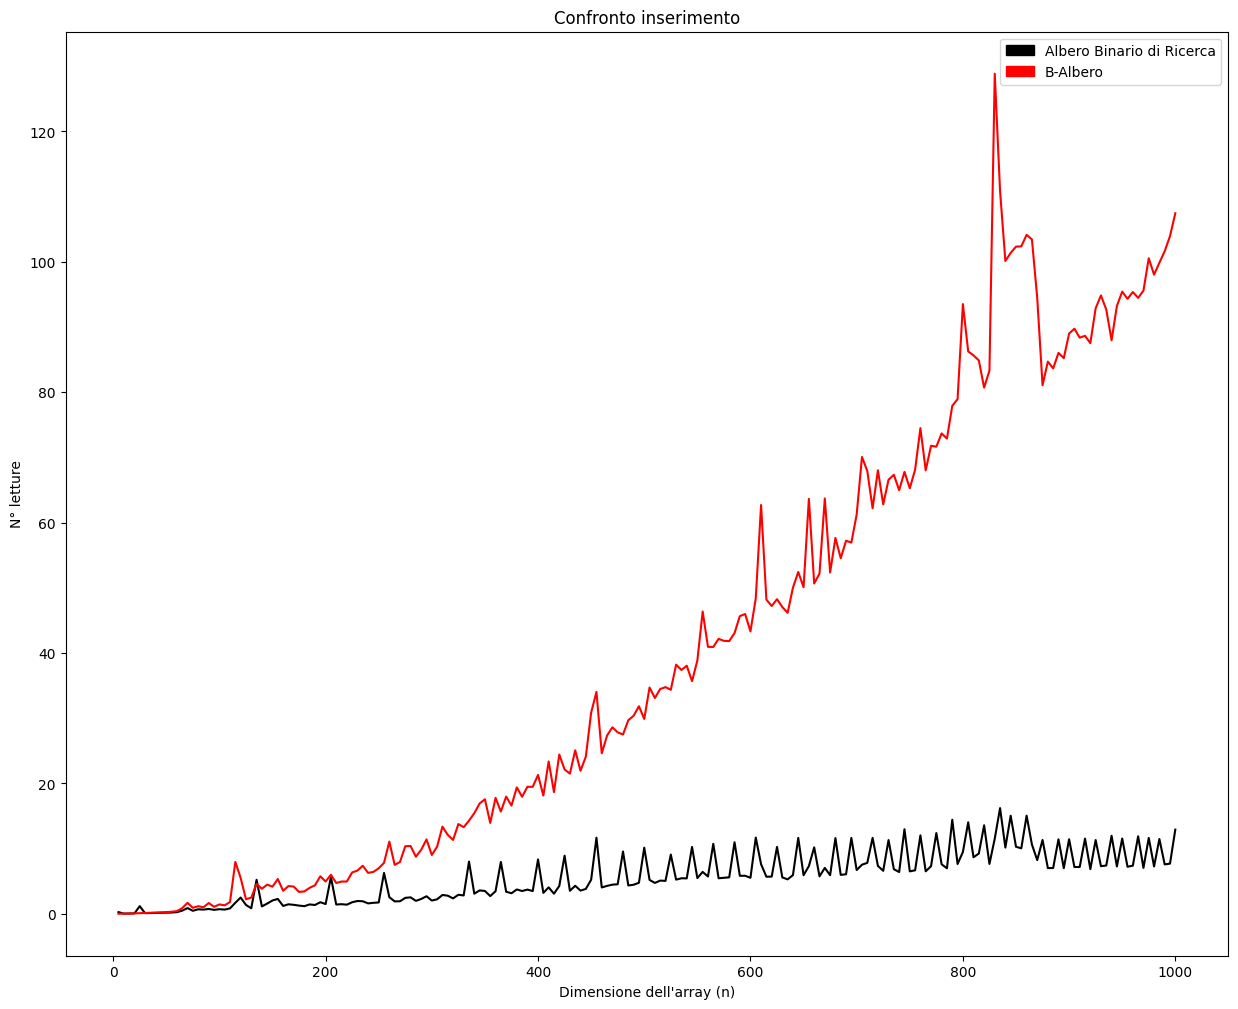
\includegraphics[width=\textwidth]{comparison-graphs/insert-ms-t100.png}
        \caption{Inserimento}
        \label{fig:compgraphinserttimet100}
    \end{subfigure}
    \hfill
    \begin{subfigure}[b]{0.49\textwidth}
        \centering
        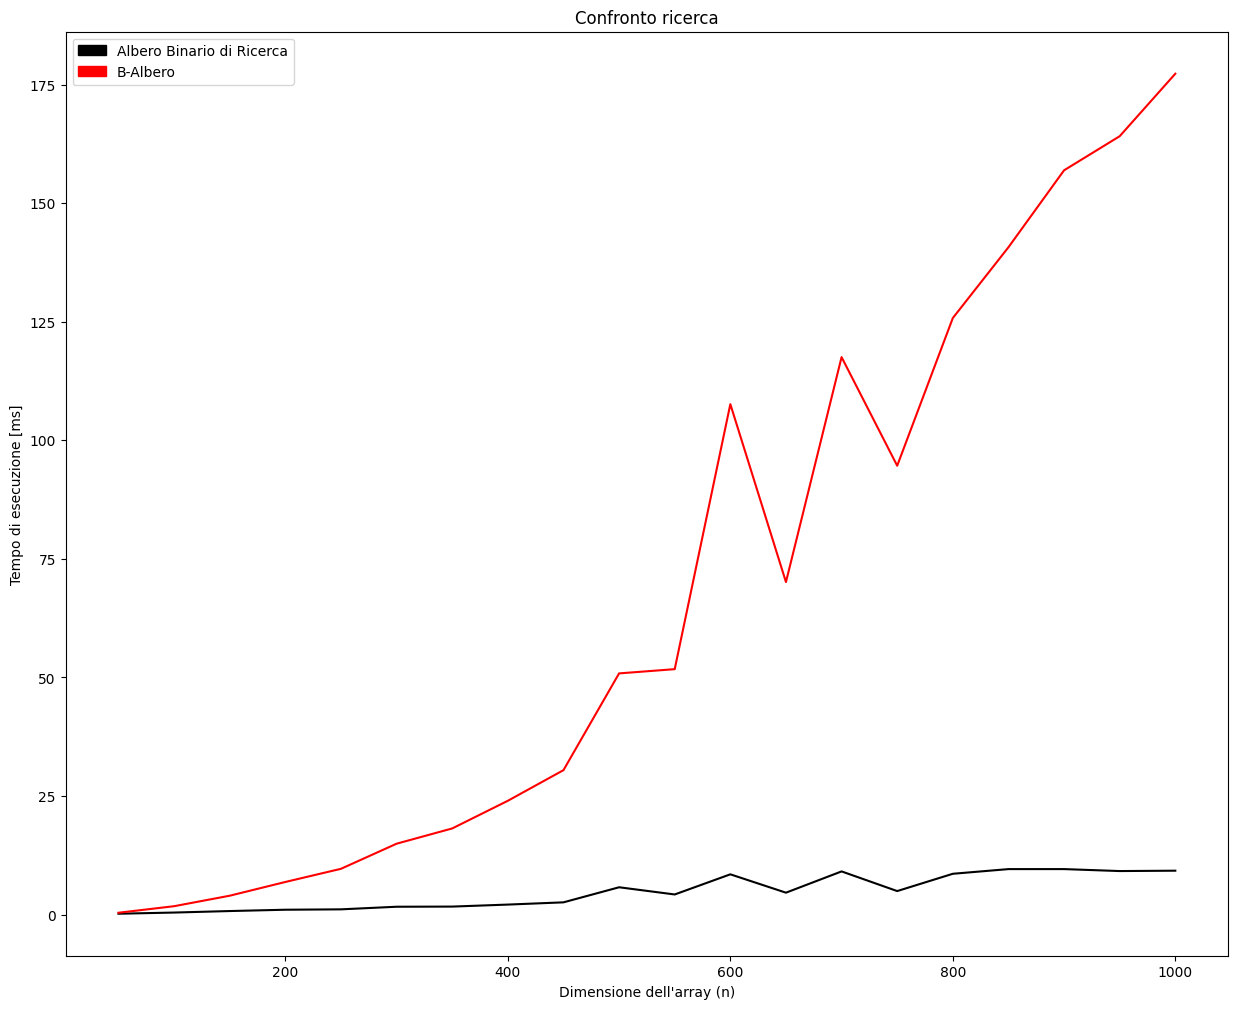
\includegraphics[width=\textwidth]{comparison-graphs/search-ms-t100.png}
        \caption{Ricerca}
        \label{fig:compgraphsearchtimet100}
    \end{subfigure}
    \caption{Grafici di confronto dei tempi con $t=100$}
    \label{fig:compgraphtimest100}
\end{figure}

\subsubsection{Alberi a confronto nei tempi con $t = 250$}
\begin{comment}
\begin{figure}[H]
    \centering
    \begin{subfigure}[b]{0.49\textwidth}
        \centering
        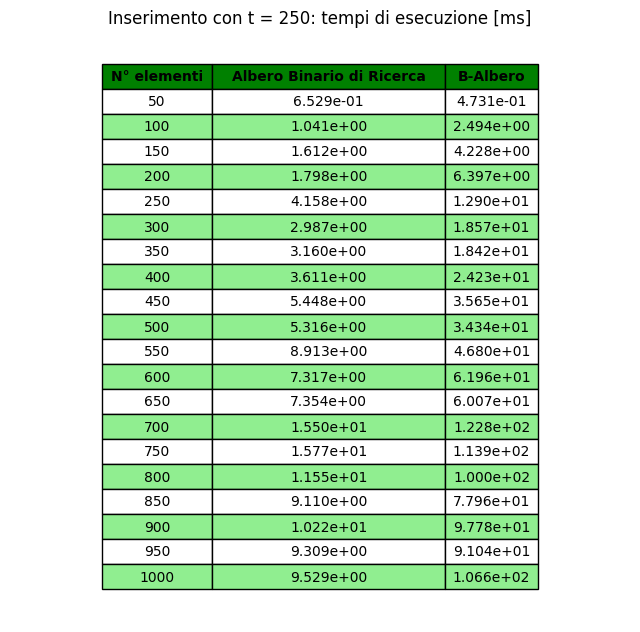
\includegraphics[width=\textwidth]{tables/insert-ms-t250.png}
        \caption{Inserimento}
        \label{fig:tableinserttimet250}
    \end{subfigure}
    \hfill
    \begin{subfigure}[b]{0.49\textwidth}
        \centering
        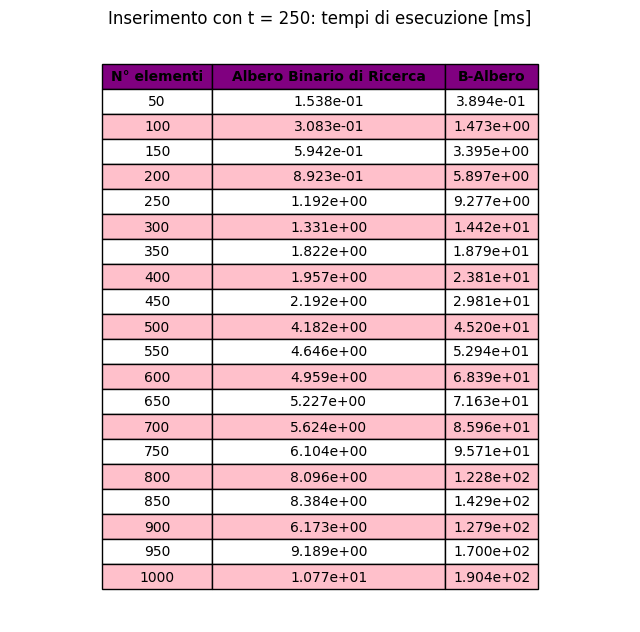
\includegraphics[width=\textwidth]{tables/search-ms-t250.png}
        \caption{Ricerca}
        \label{fig:tablesearchtimet250}
    \end{subfigure}
    \caption{Tabella tempi con $t=250$}
    \label{fig:tabletimest250}
\end{figure}
\end{comment}

\begin{figure}[H]
    \centering
    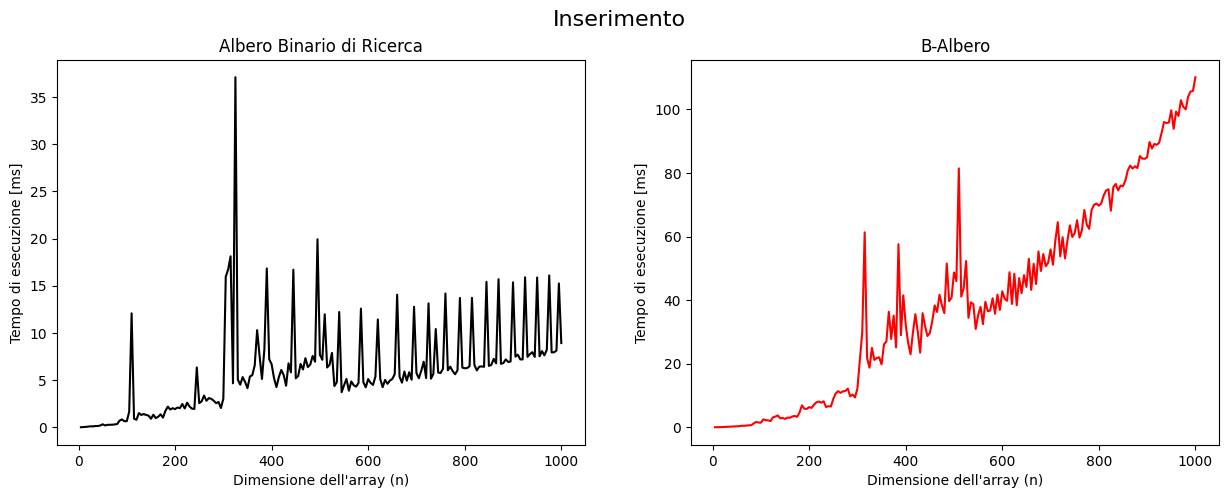
\includegraphics[width=\textwidth]{side-graphs/insert-ms-t250.png}
    \caption{Grafico tempi dell'Inserimento con $t=250$}
    \label{fig:sidegraphinserttimet250}
\end{figure}
    
\begin{figure}[H]
    \centering
    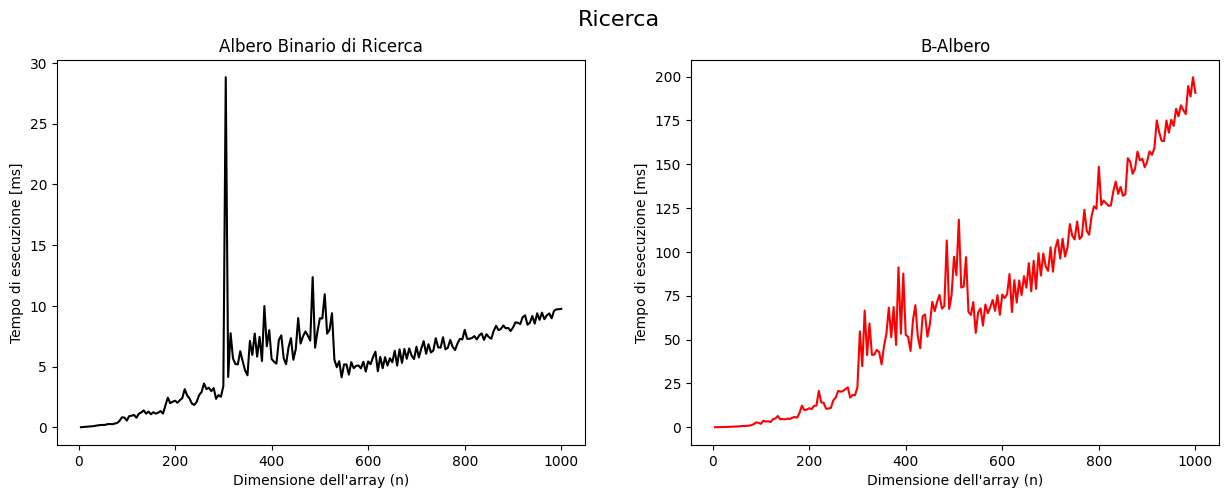
\includegraphics[width=\textwidth]{side-graphs/search-ms-t250.png}
    \caption{Grafico tempi della Ricerca con $t=250$}    
    \label{fig:sidegraphsearchtimet250}
\end{figure}

\begin{figure}[H]
    \centering
    \begin{subfigure}[b]{0.49\textwidth}
        \centering
        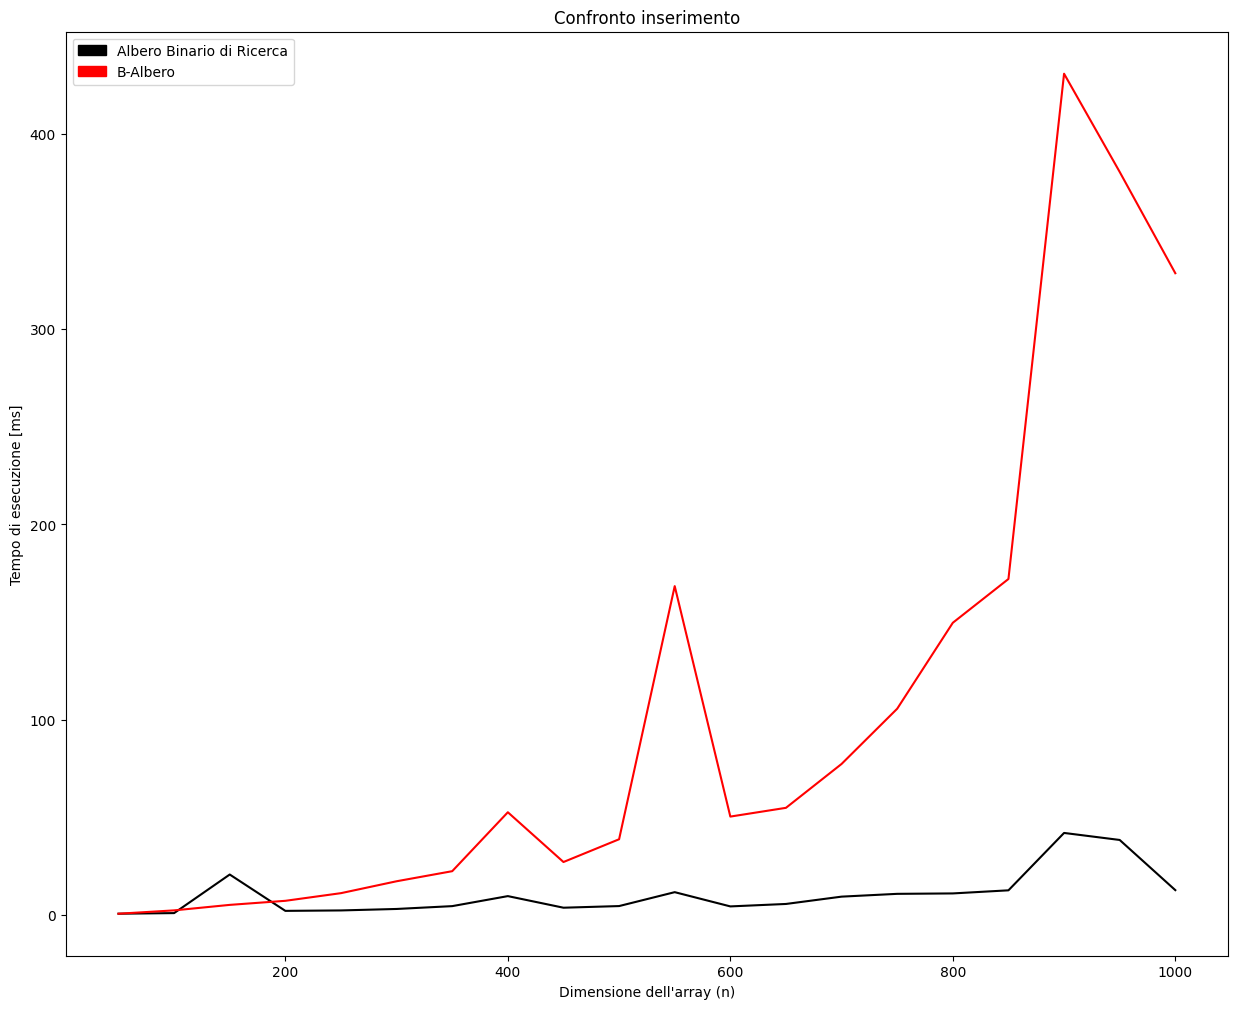
\includegraphics[width=\textwidth]{comparison-graphs/insert-ms-t250.png}
        \caption{Inserimento}
        \label{fig:compgraphinserttimet250}
    \end{subfigure}
    \hfill
    \begin{subfigure}[b]{0.49\textwidth}
        \centering
        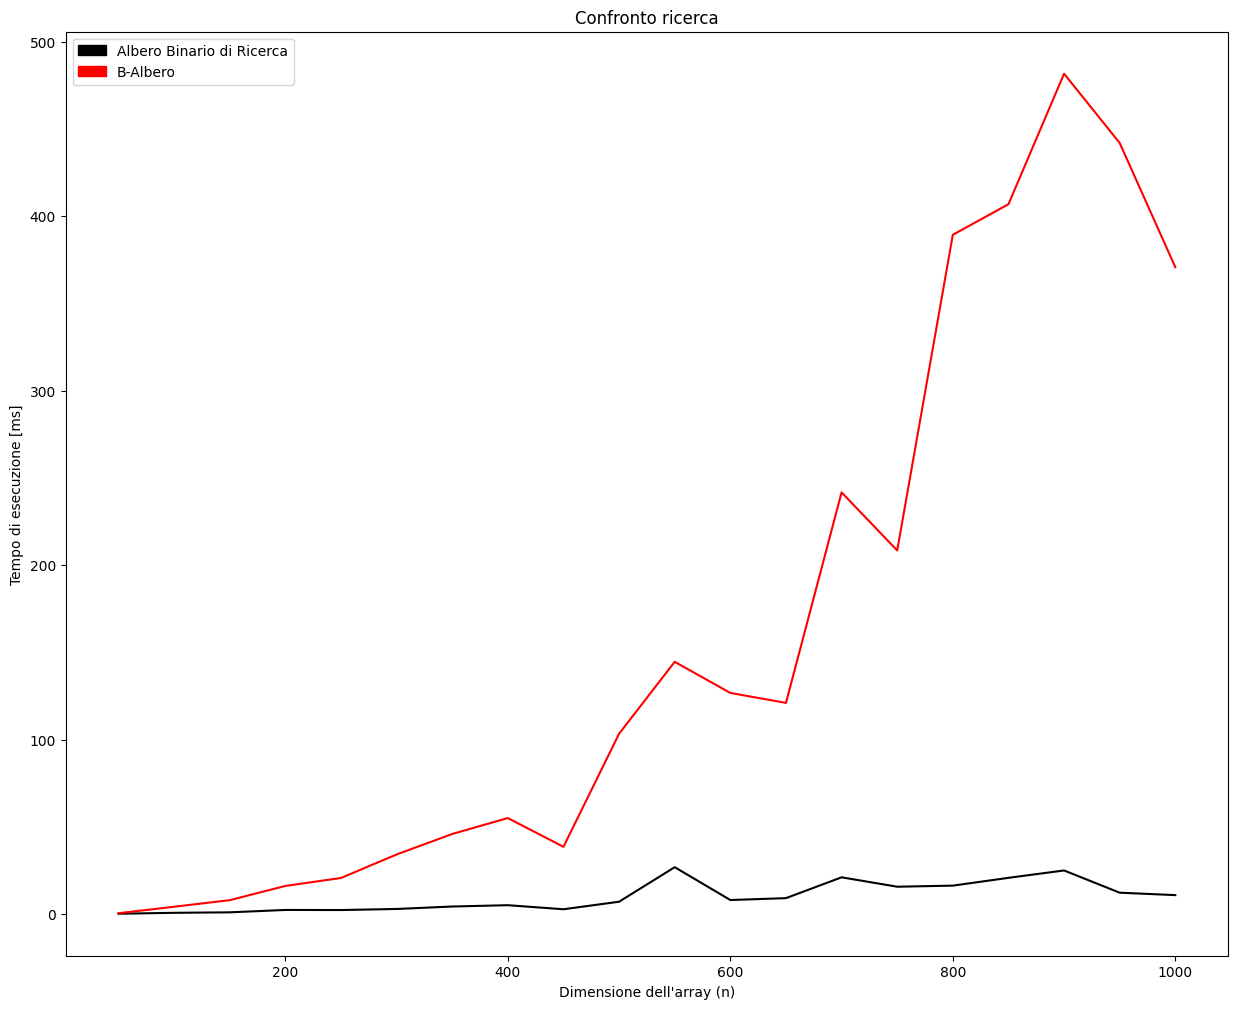
\includegraphics[width=\textwidth]{comparison-graphs/search-ms-t250.png}
        \caption{Ricerca}
        \label{fig:compgraphsearchtimet250}
    \end{subfigure}
    \caption{Grafici di confronto dei tempi con $t=250$}
    \label{fig:compgraphtimest250}
\end{figure}


\subsubsection{Alberi a confronto nei tempi con $t = 1000$}
\begin{comment}
\begin{figure}[H]
    \centering
    \begin{subfigure}[b]{0.49\textwidth}
        \centering
        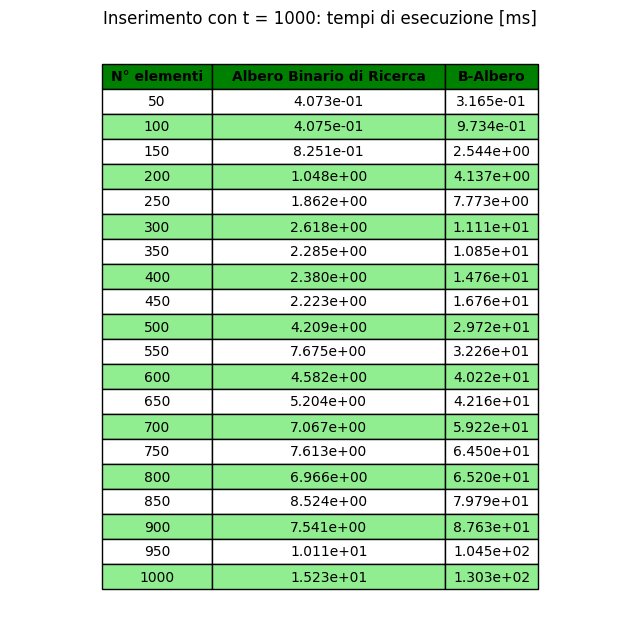
\includegraphics[width=\textwidth]{tables/insert-ms-t1000.png}
        \caption{Inserimento}
        \label{fig:tableinserttimet1000}
    \end{subfigure}
    \hfill
    \begin{subfigure}[b]{0.49\textwidth}
        \centering
        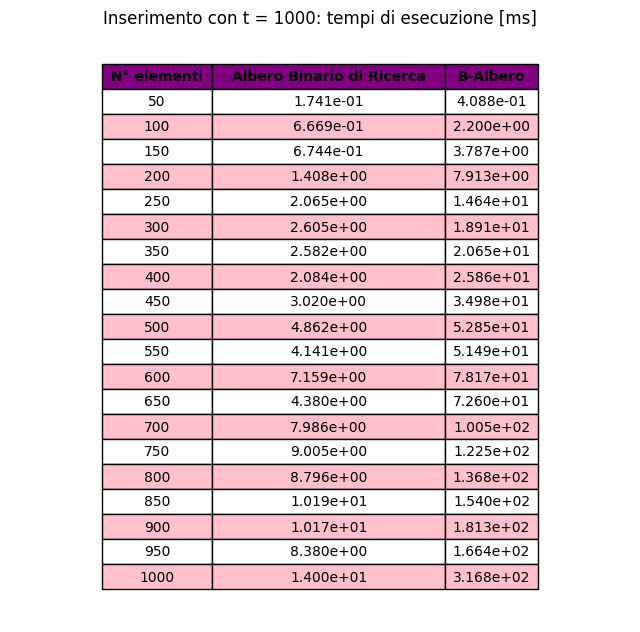
\includegraphics[width=\textwidth]{tables/search-ms-t1000.png}
        \caption{Ricerca}
        \label{fig:tablesearchtimet1000}
    \end{subfigure}
    \caption{Tabella tempi con $t=1000$}
    \label{fig:tabletimest1000}
\end{figure}
\end{comment}

\begin{figure}[H]
    \centering
    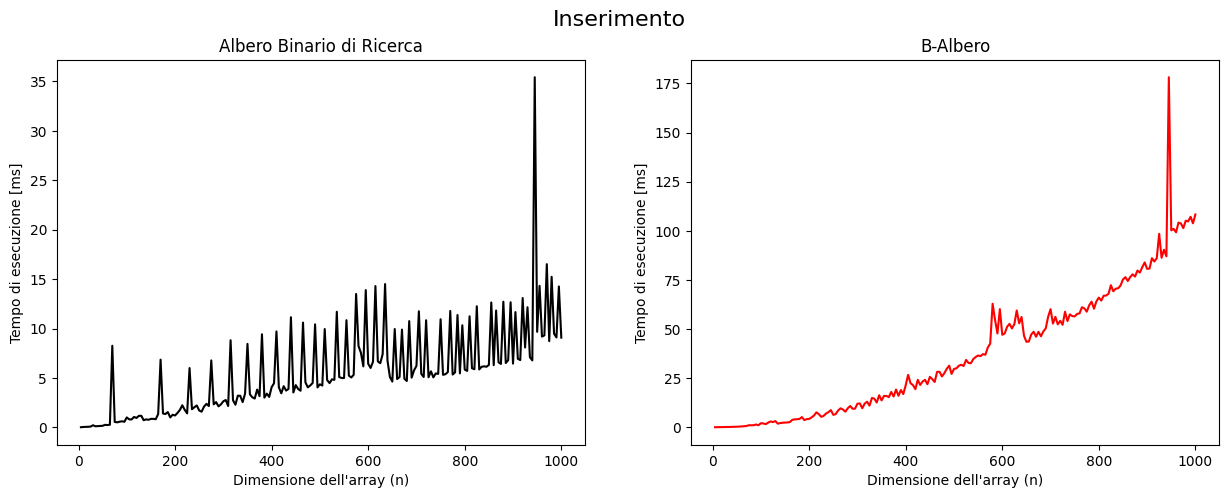
\includegraphics[width=\textwidth]{side-graphs/insert-ms-t1000.png}
    \caption{Grafico tempi dell'Inserimento con $t=1000$}
    \label{fig:sidegraphinserttimet1000}
\end{figure}
    
\begin{figure}[H]
    \centering
    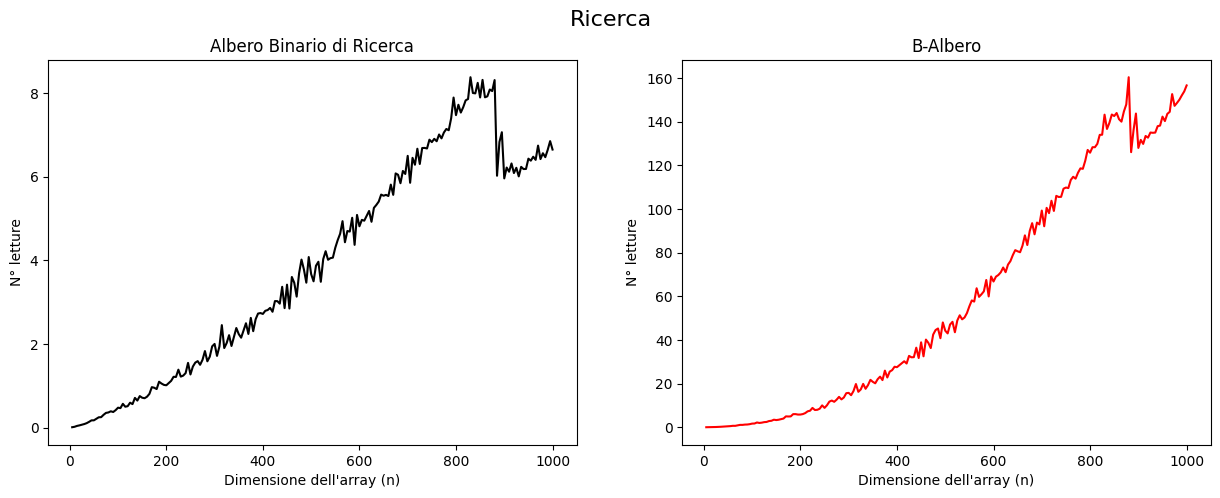
\includegraphics[width=\textwidth]{side-graphs/search-ms-t1000.png}
    \caption{Grafico tempi della Ricerca con $t=1000$}    
    \label{fig:sidegraphsearchtimet1000}
\end{figure}

\begin{figure}[H]
    \centering
    \begin{subfigure}[b]{0.49\textwidth}
        \centering
        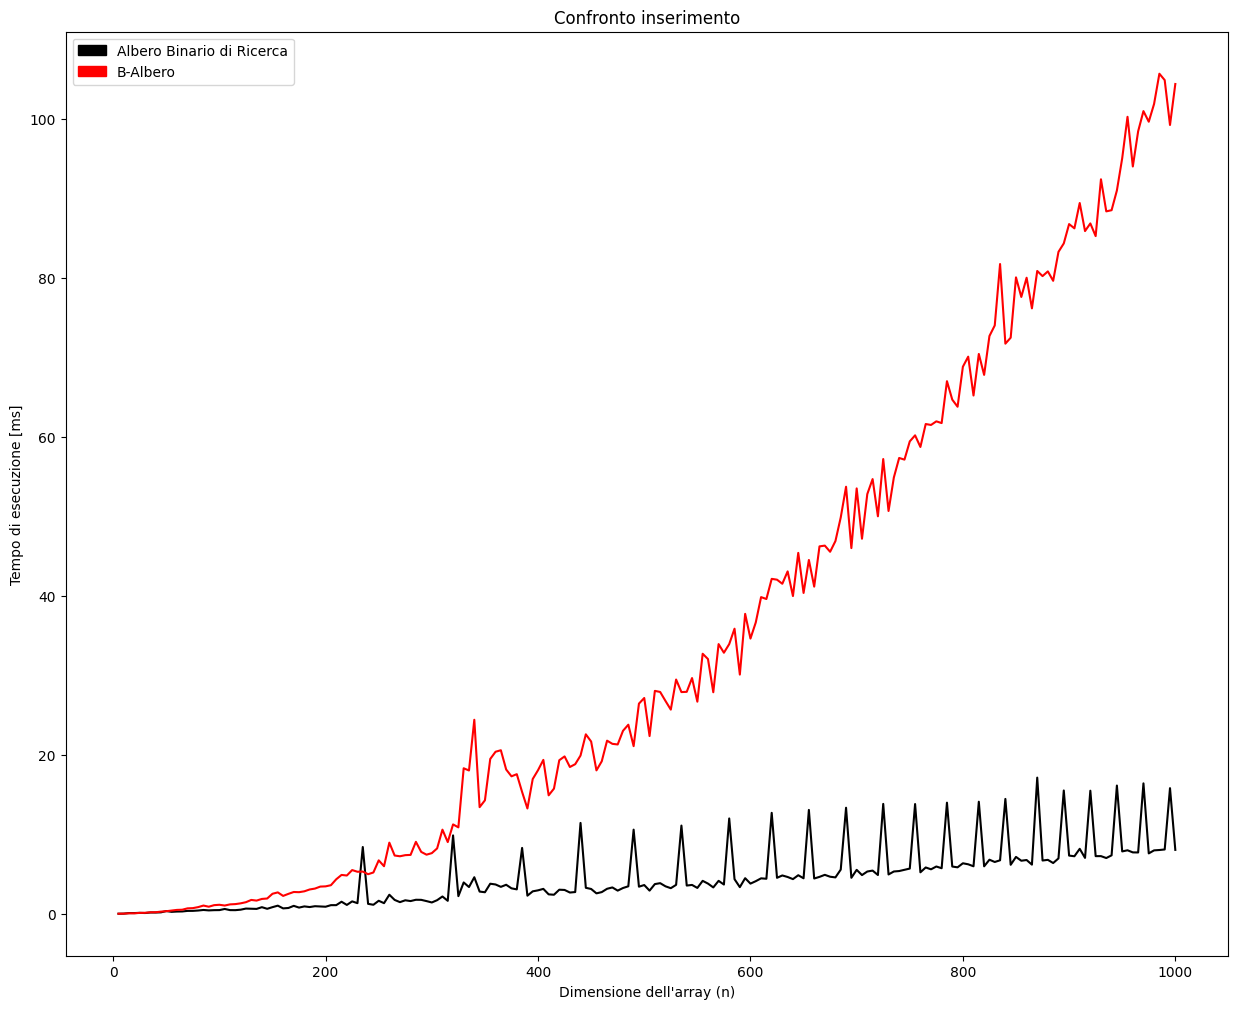
\includegraphics[width=\textwidth]{comparison-graphs/insert-ms-t1000.png}
        \caption{Inserimento}
        \label{fig:compgraphinserttimet1000}
    \end{subfigure}
    \hfill
    \begin{subfigure}[b]{0.49\textwidth}
        \centering
        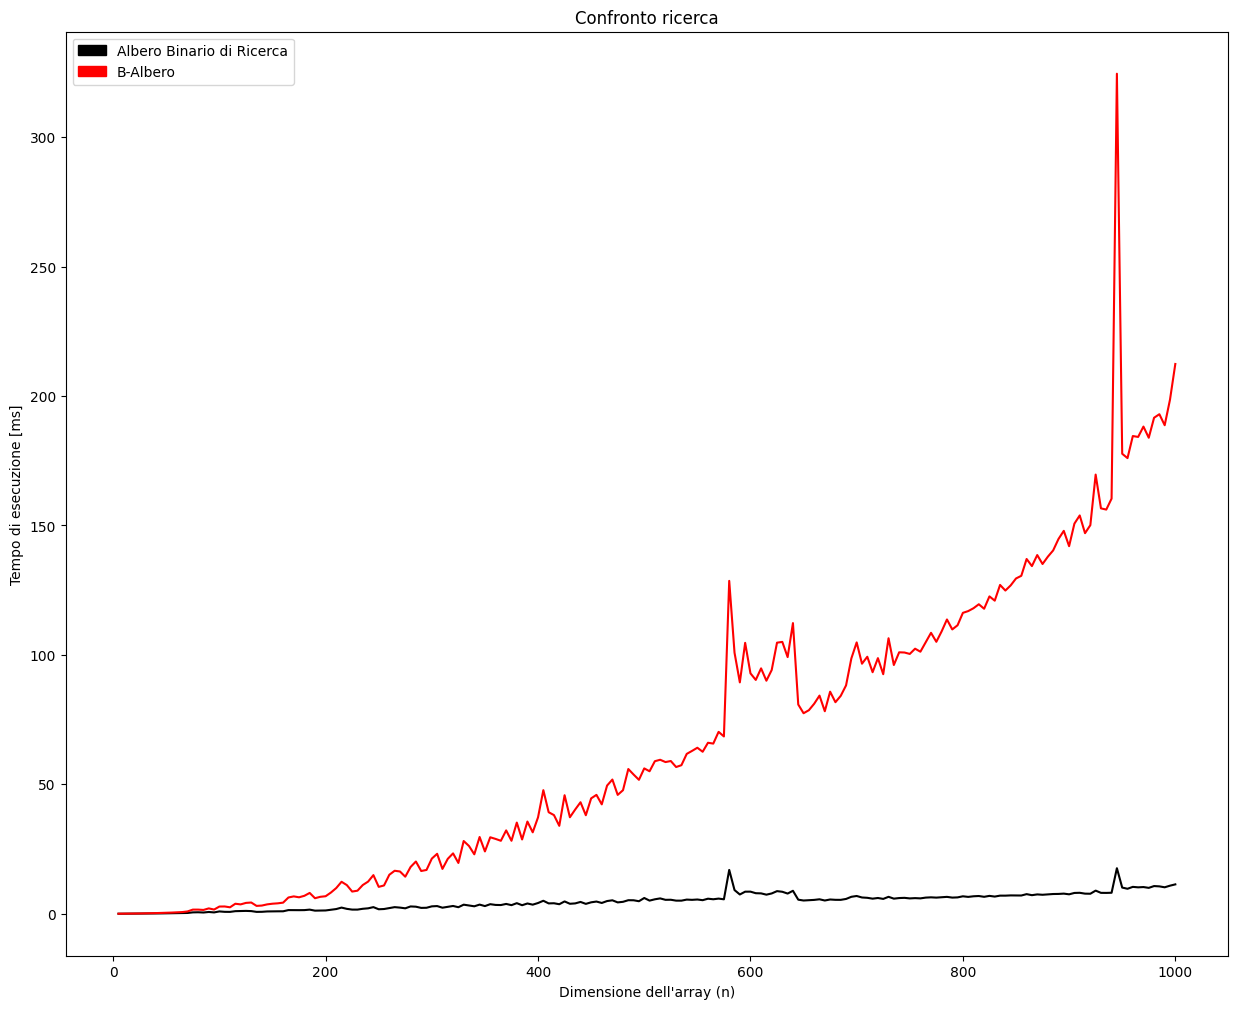
\includegraphics[width=\textwidth]{comparison-graphs/search-ms-t1000.png}
        \caption{Ricerca}
        \label{fig:compgraphsearchtimet1000}
    \end{subfigure}
    \caption{Grafici di confronto dei tempi con $t=1000$}
    \label{fig:compgraphtimest1000}
\end{figure}


\textbf{Ora invece guardo il numero di letture e scritture:}

\subsubsection{Alberi a confronto nel numero di letture e scritture con $t = 100$}

\begin{comment}
\begin{figure}[H]
    \centering
    \begin{subfigure}[b]{0.49\textwidth}
        \centering
        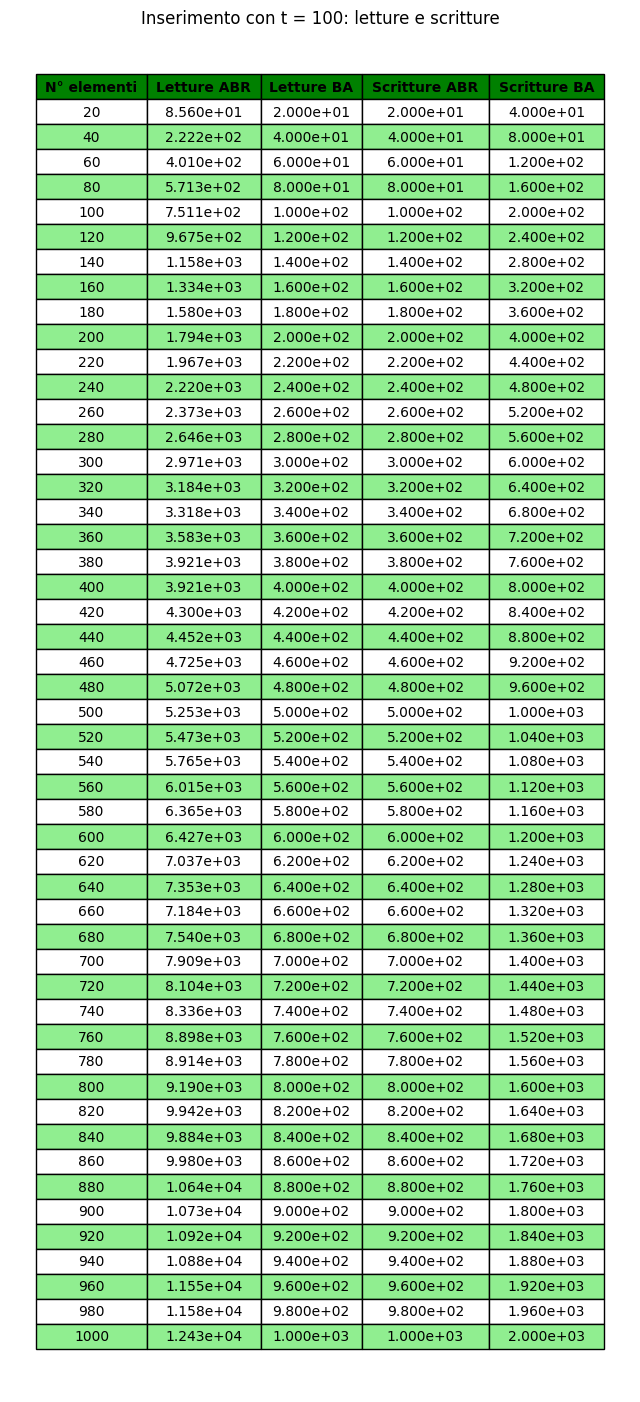
\includegraphics[width=\textwidth]{tables/insert-wr-t100.png}
        \caption{Inserimento, letture e scritture}
        \label{fig:tableinsertwr100}
    \end{subfigure}
    \hfill
    \begin{subfigure}[b]{0.49\textwidth}
        \centering
        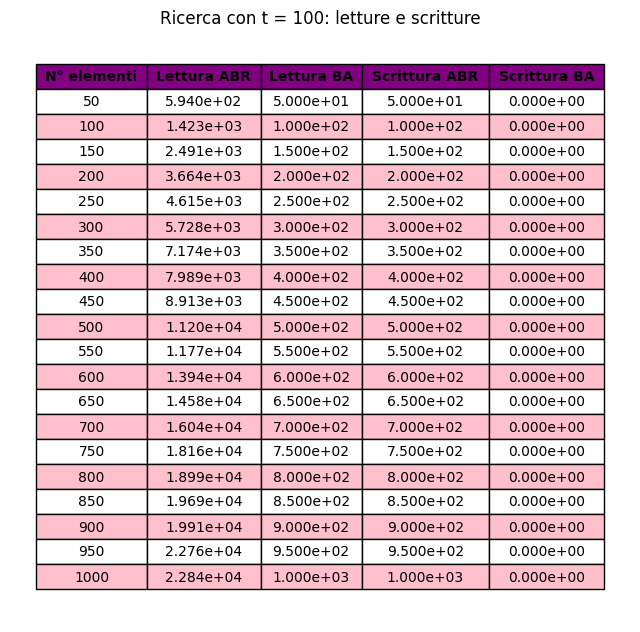
\includegraphics[width=\textwidth]{tables/search-wr-t100.png}
        \caption{Ricerca, letture e scritture}
        \label{fig:tablesearchwr100}
    \end{subfigure}
    \caption{Tabelle scritture e letture con $t=100$}
    \label{fig:tablewr100}
\end{figure}
\end{comment}

\begin{figure}[H]
    \centering
    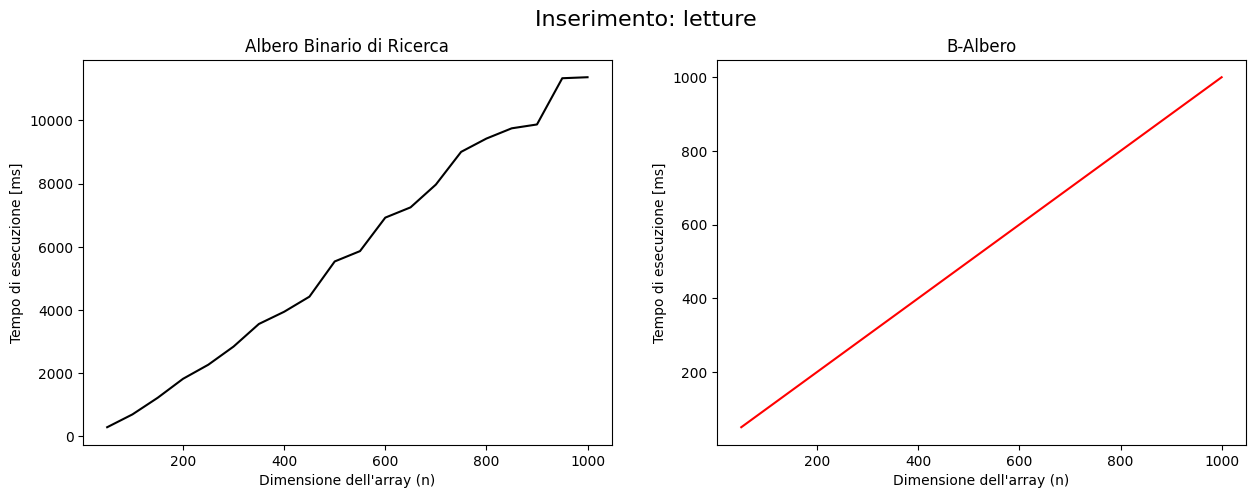
\includegraphics[width=\textwidth]{side-graphs/insert-r-t100.png}
    \caption{Grafico delle letture dell'Inserimento con $t=100$}
    \label{fig:sidegraphinsertread100}
\end{figure}
    
\begin{figure}[H]
    \centering
    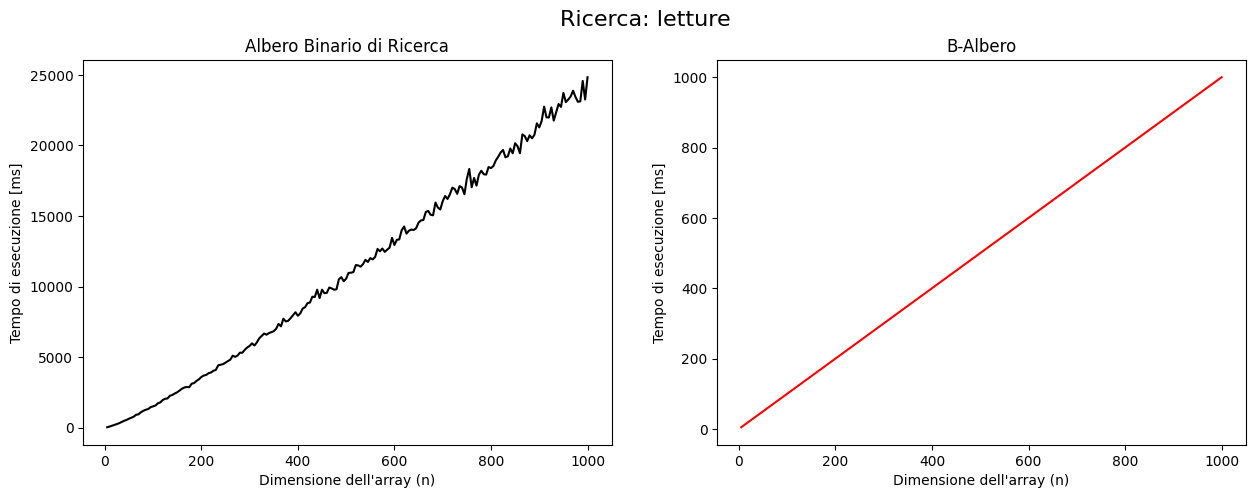
\includegraphics[width=\textwidth]{side-graphs/search-r-t100.png}
    \caption{Grafico delle letture della Ricerca con $t=100$}
    \label{fig:sidegraphsearchread100}
\end{figure}

\begin{figure}[H]
    \centering
    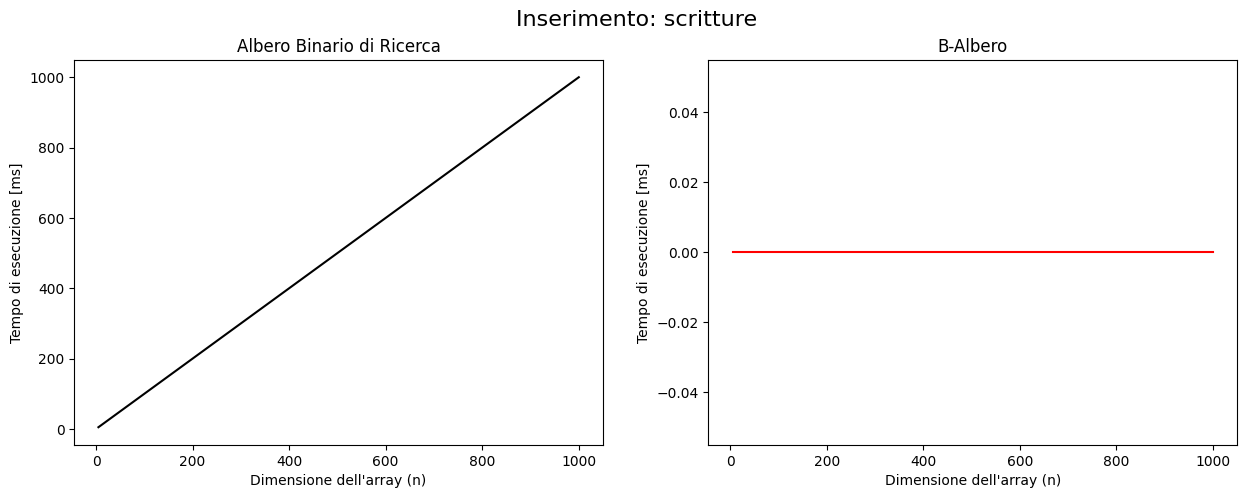
\includegraphics[width=\textwidth]{side-graphs/insert-w-t100.png}
    \caption{Grafico delle scritture dell'Inserimento con $t=100$}
    \label{fig:sidegraphinsertwrite100}
\end{figure}
    
\begin{figure}[H]
    \centering
    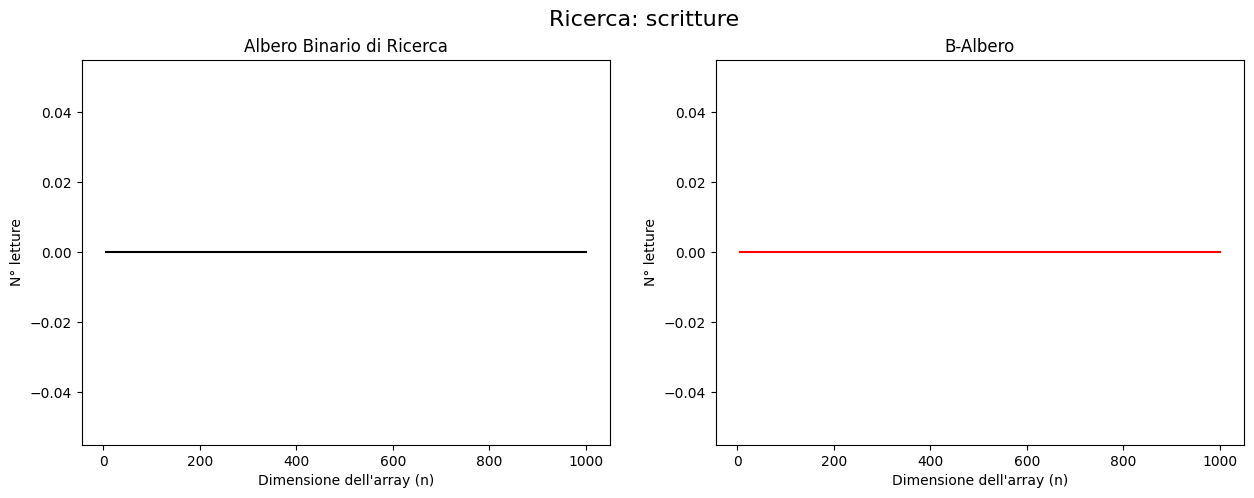
\includegraphics[width=\textwidth]{side-graphs/search-w-t100.png}
    \caption{Grafico delle scritture della Ricerca con $t=100$}
    \label{fig:sidegraphsearchwrite100}
\end{figure}

\begin{figure}[H]
    \centering
    \begin{subfigure}[b]{0.49\textwidth}
        \centering
        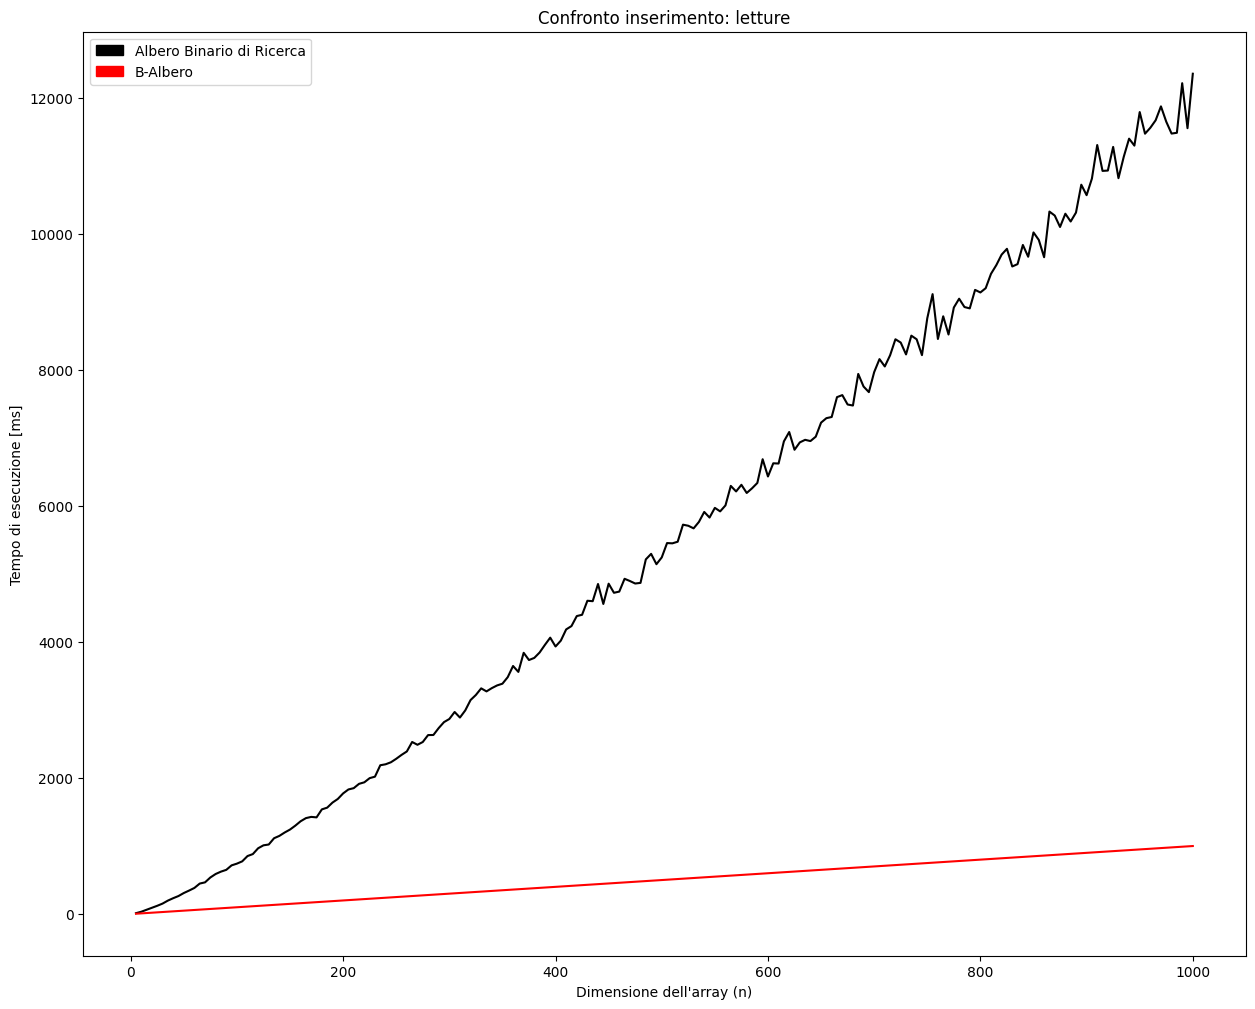
\includegraphics[width=\textwidth]{comparison-graphs/insert-r-t100.png}
        \caption{Inserimento}
        \label{fig:compgraphinsertread100}
    \end{subfigure}
    \hfill
    \begin{subfigure}[b]{0.49\textwidth}
        \centering
        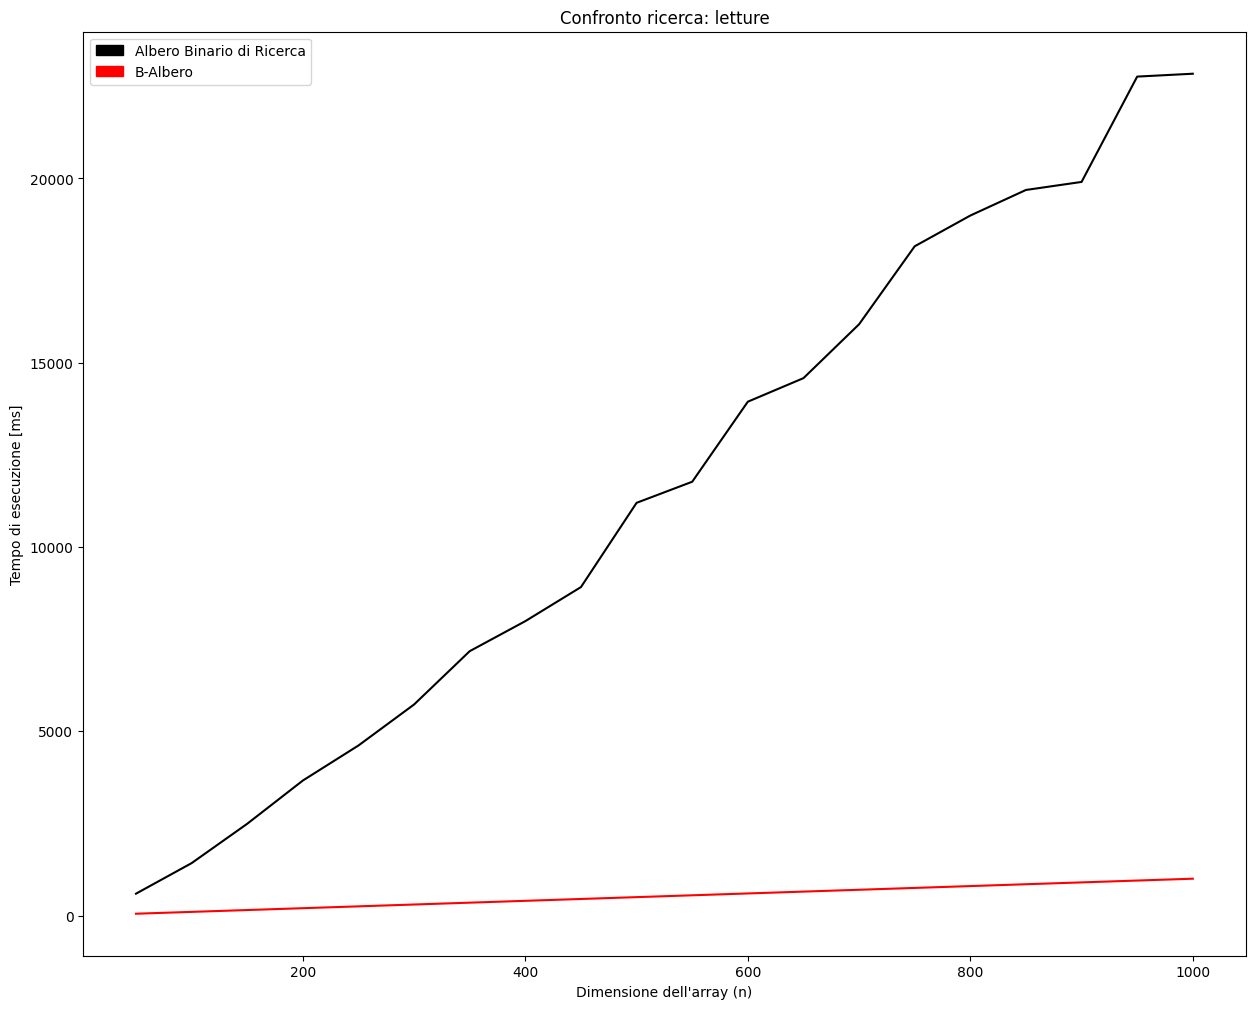
\includegraphics[width=\textwidth]{comparison-graphs/search-r-t100.png}
        \caption{Ricerca}
        \label{fig:compgraphsearchread100}
    \end{subfigure}
    \caption{Grafici di confronto delle letture con $t=100$}
    \label{fig:compgraphread100}
\end{figure}

\begin{figure}[H]
    \centering
    \begin{subfigure}[b]{0.49\textwidth}
        \centering
        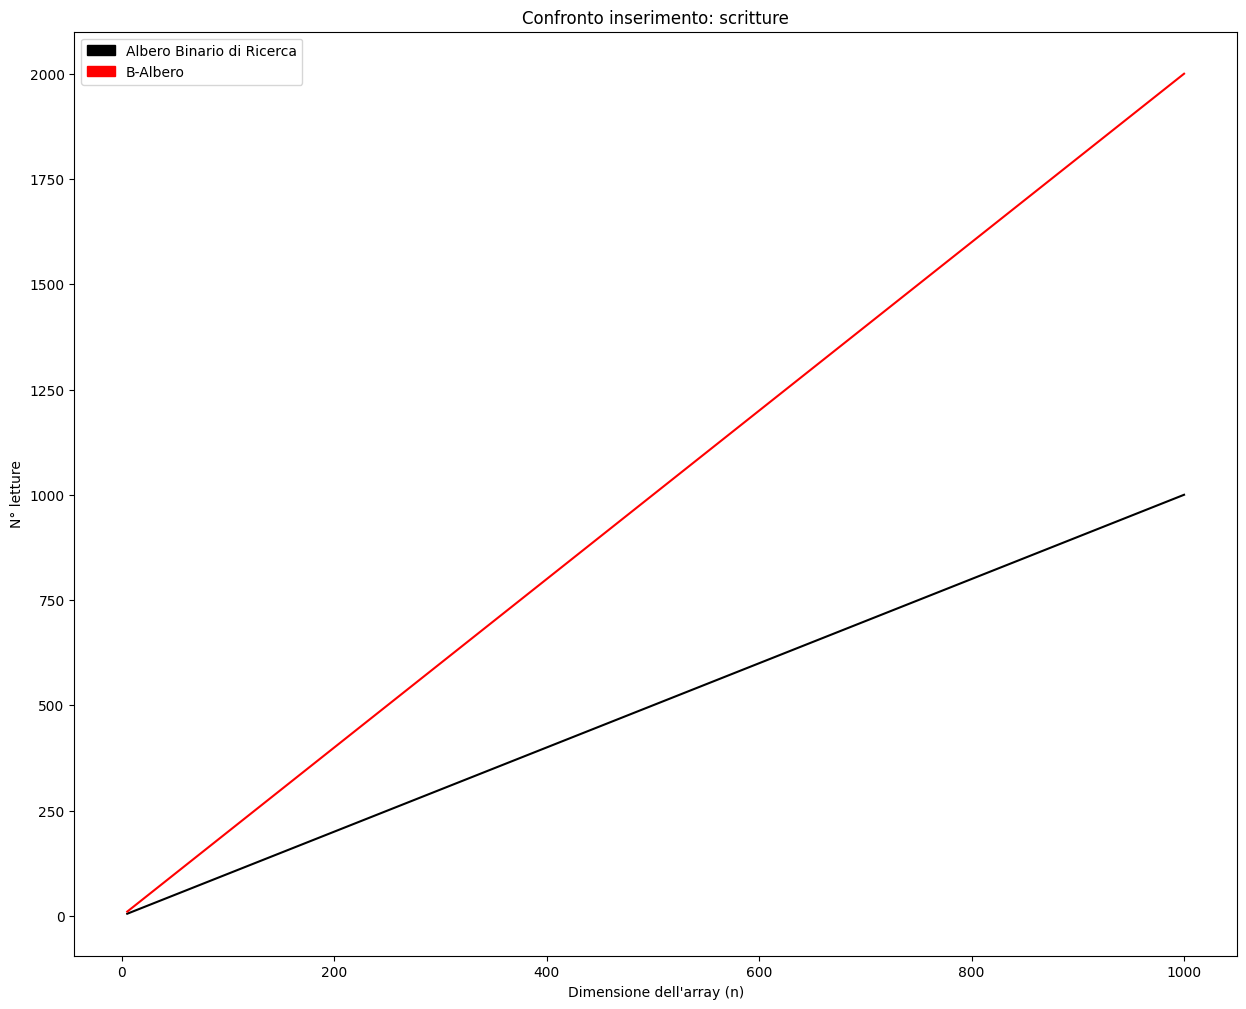
\includegraphics[width=\textwidth]{comparison-graphs/insert-w-t100.png}
        \caption{Inserimento}
        \label{fig:compgraphinsertwrite100}
    \end{subfigure}
    \hfill
    \begin{subfigure}[b]{0.49\textwidth}
        \centering
        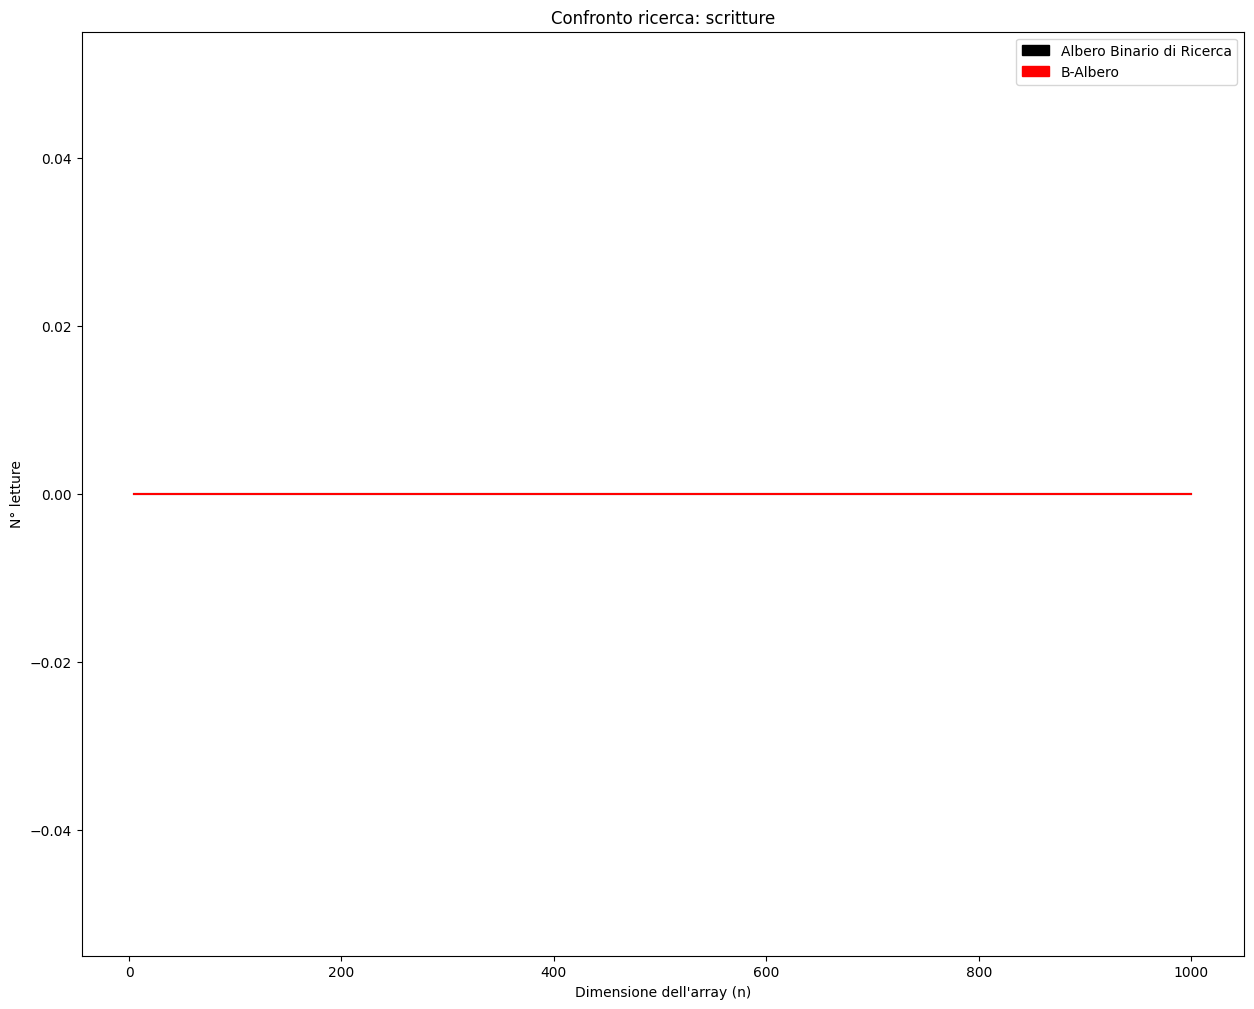
\includegraphics[width=\textwidth]{comparison-graphs/search-w-t100.png}
        \caption{Ricerca}
        \label{fig:compgraphsearchwrite100}
    \end{subfigure}
    \caption{Grafici di confronto delle scritture con $t=100$}
    \label{fig:compgraphread100}
\end{figure}



\subsubsection{Alberi a confronto nel numero di letture e scritture con $t = 250$}

\begin{comment}
\begin{figure}[H]
    \centering
    \begin{subfigure}[b]{0.49\textwidth}
        \centering
        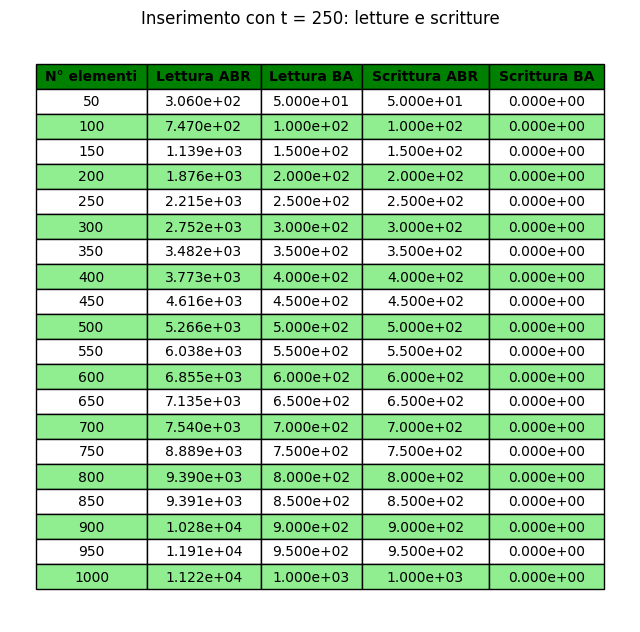
\includegraphics[width=\textwidth]{tables/insert-wr-t250.png}
        \caption{Inserimento, letture e scritture}
        \label{fig:tableinsertwr250}
    \end{subfigure}
    \hfill
    \begin{subfigure}[b]{0.49\textwidth}
        \centering
        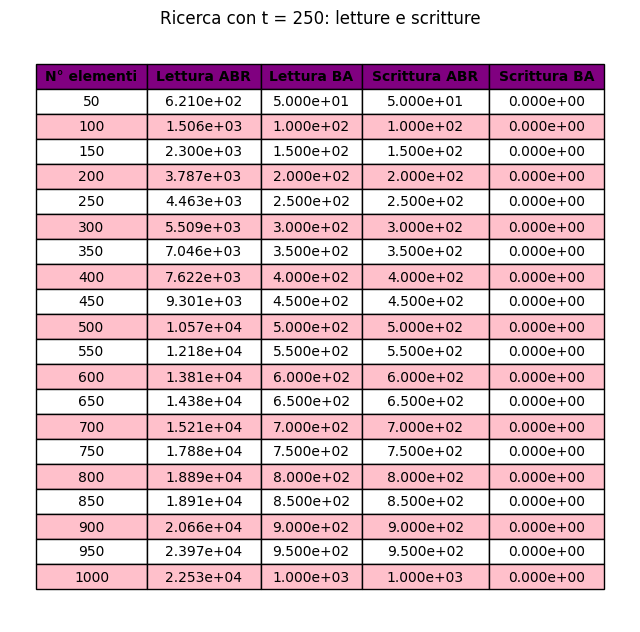
\includegraphics[width=\textwidth]{tables/search-wr-t250.png}
        \caption{Ricerca, letture e scritture}
        \label{fig:tablesearchwr250}
    \end{subfigure}
    \caption{Tabelle scritture e letture con $t=250$}
    \label{fig:tablewr250}
\end{figure}
\end{comment}

\begin{figure}[H]
    \centering
    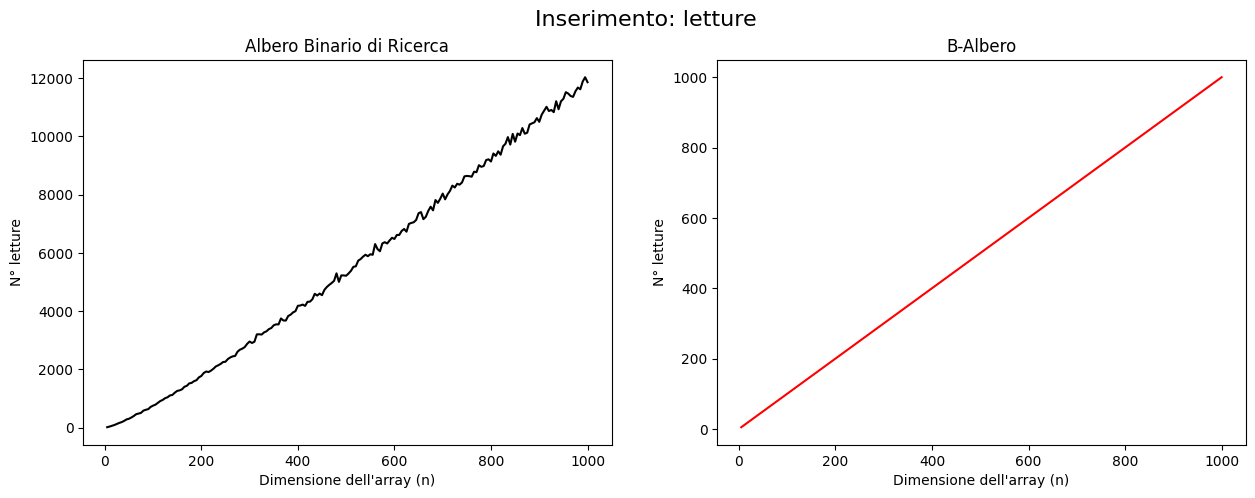
\includegraphics[width=\textwidth]{side-graphs/insert-r-t250.png}
    \caption{Grafico delle letture dell'Inserimento con $t=250$}
    \label{fig:sidegraphinsertread250}
\end{figure}
    
\begin{figure}[H]
    \centering
    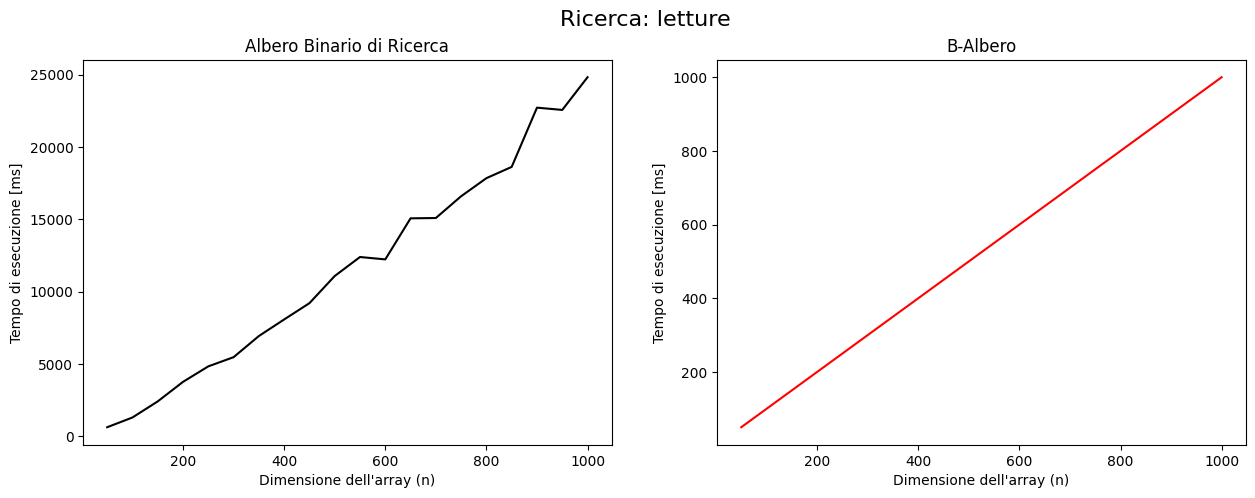
\includegraphics[width=\textwidth]{side-graphs/search-r-t250.png}
    \caption{Grafico delle letture della Ricerca con $t=250$}
    \label{fig:sidegraphsearchread250}
\end{figure}

\begin{figure}[H]
    \centering
    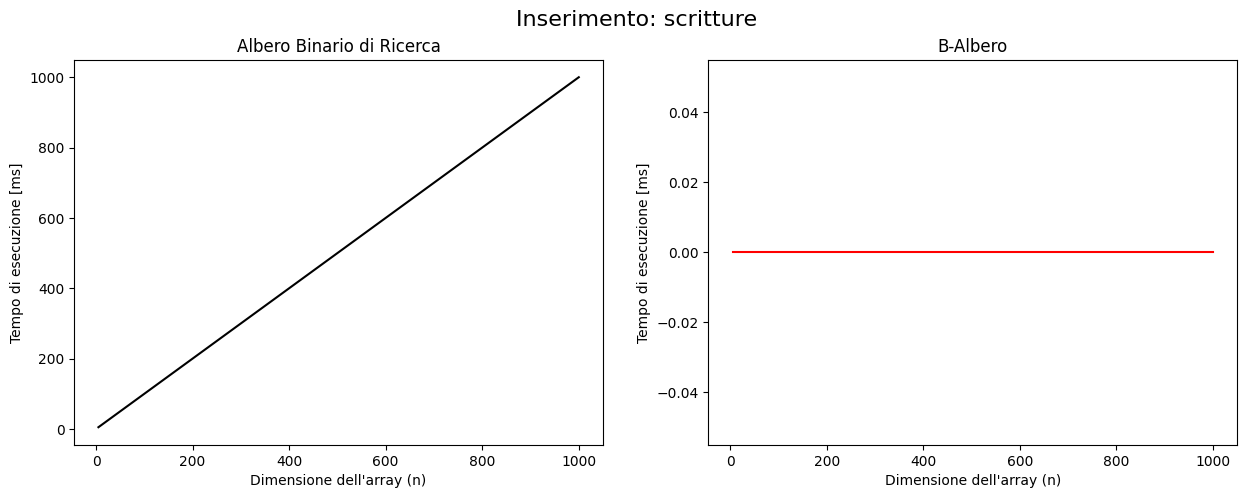
\includegraphics[width=\textwidth]{side-graphs/insert-w-t250.png}
    \caption{Grafico delle scritture dell'Inserimento con $t=250$}
    \label{fig:sidegraphinsertwrite250}
\end{figure}
    
\begin{figure}[H]
    \centering
    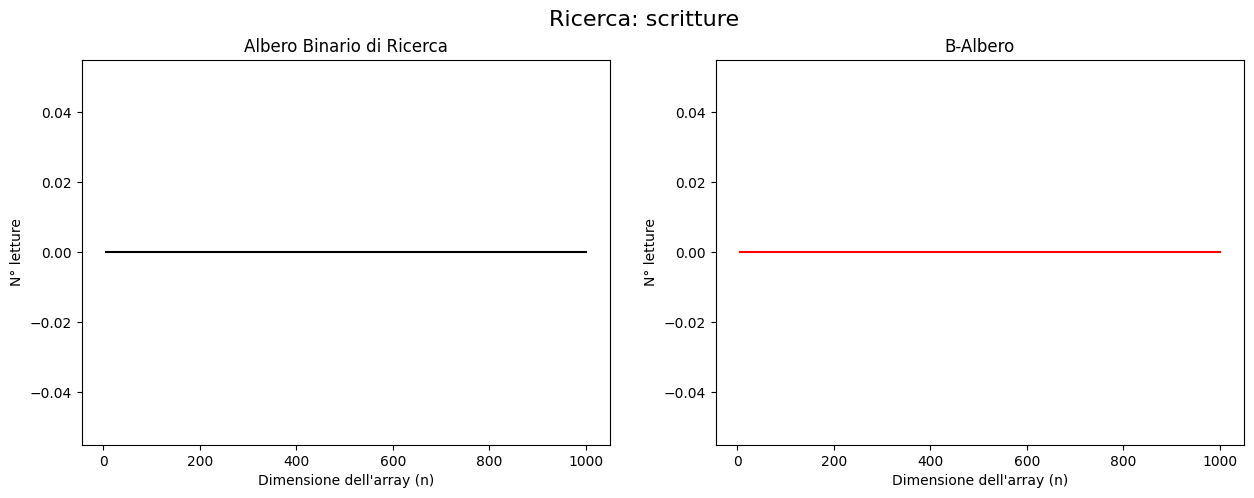
\includegraphics[width=\textwidth]{side-graphs/search-w-t250.png}
    \caption{Grafico delle scritture della Ricerca con $t=250$}
    \label{fig:sidegraphsearchwrite250}
\end{figure}

\begin{figure}[H]
    \centering
    \begin{subfigure}[b]{0.49\textwidth}
        \centering
        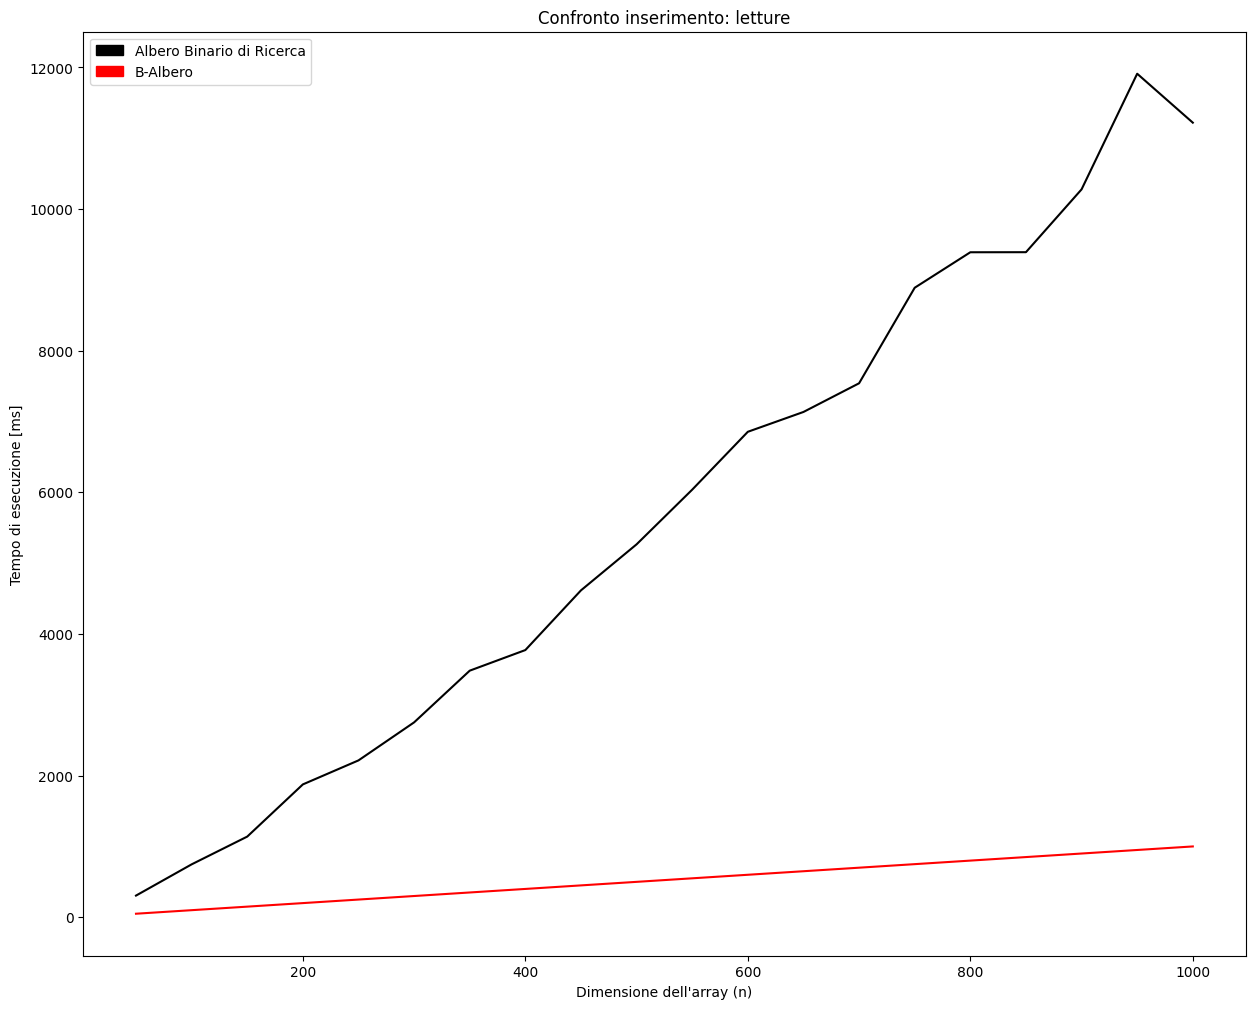
\includegraphics[width=\textwidth]{comparison-graphs/insert-r-t250.png}
        \caption{Inserimento}
        \label{fig:compgraphinsertread250}
    \end{subfigure}
    \hfill
    \begin{subfigure}[b]{0.49\textwidth}
        \centering
        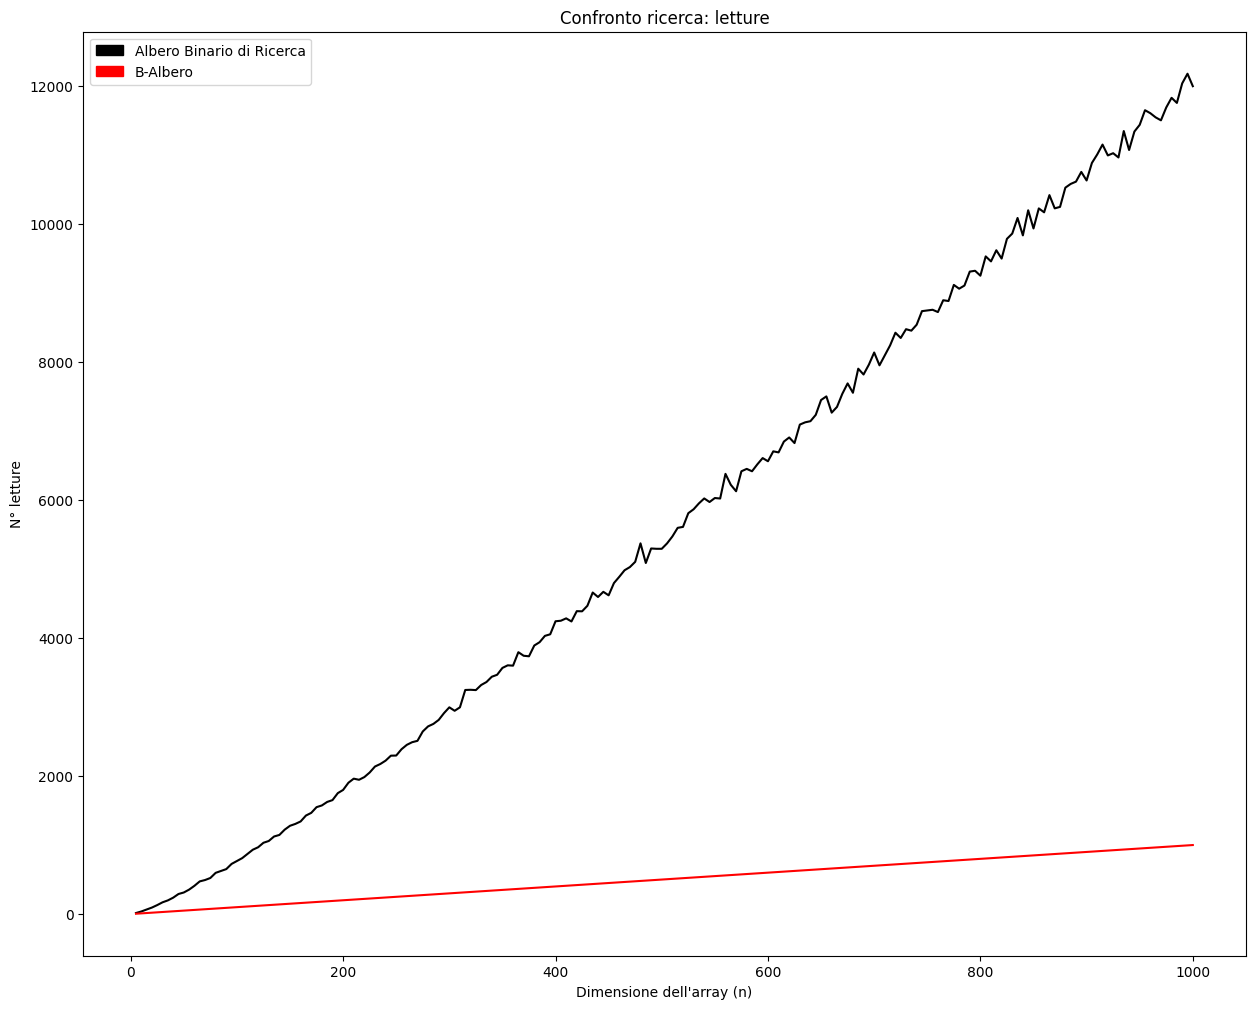
\includegraphics[width=\textwidth]{comparison-graphs/search-r-t250.png}
        \caption{Ricerca}
        \label{fig:compgraphsearchread250}
    \end{subfigure}
    \caption{Grafici di confronto delle letture con $t=250$}
    \label{fig:compgraphread250}
\end{figure}

\begin{figure}[H]
    \centering
    \begin{subfigure}[b]{0.49\textwidth}
        \centering
        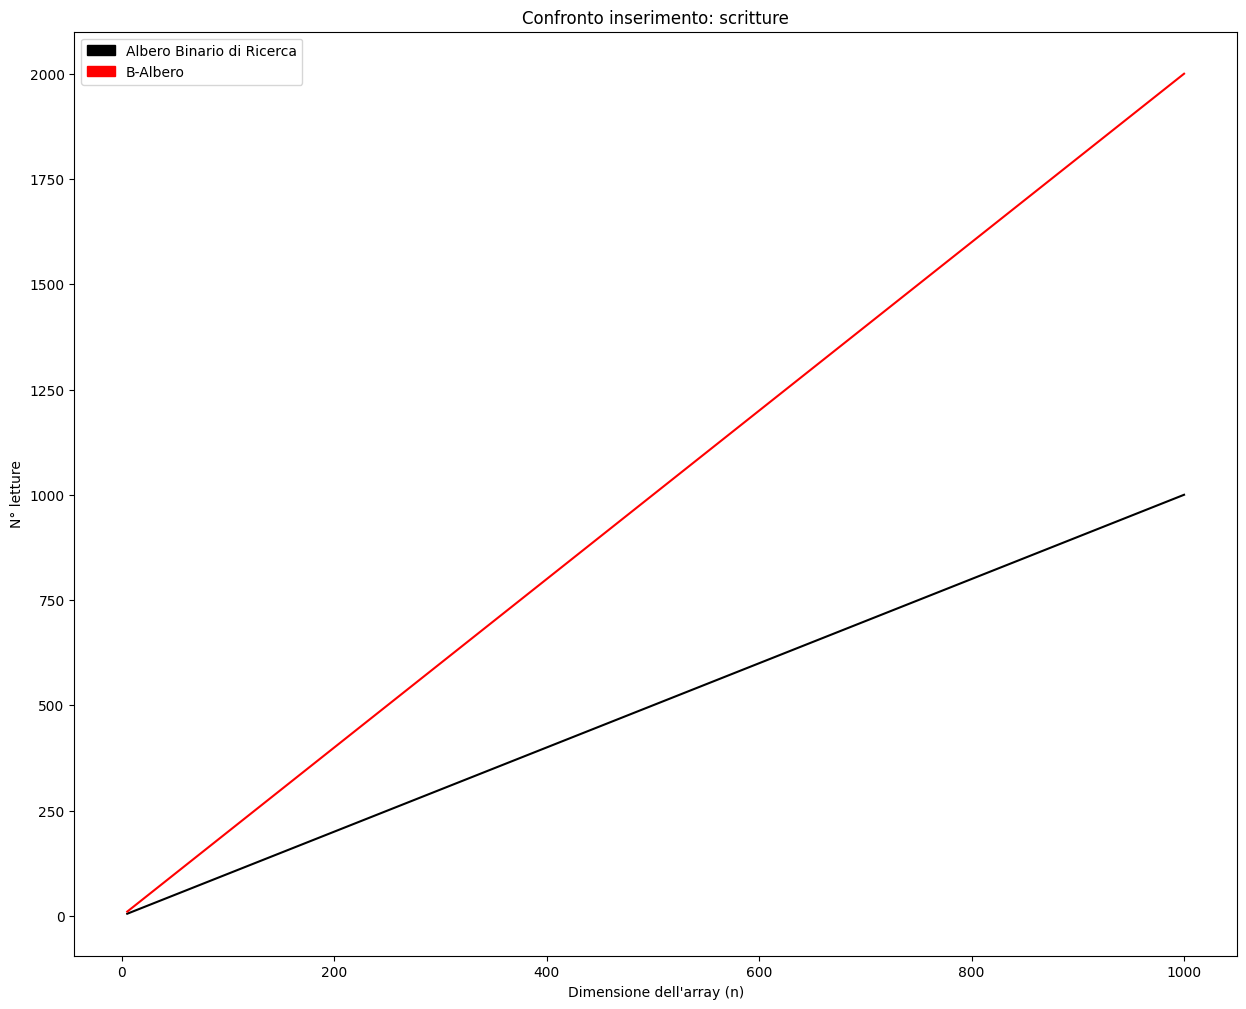
\includegraphics[width=\textwidth]{comparison-graphs/insert-w-t250.png}
        \caption{Inserimento}
        \label{fig:compgraphinsertwrite250}
    \end{subfigure}
    \hfill
    \begin{subfigure}[b]{0.49\textwidth}
        \centering
        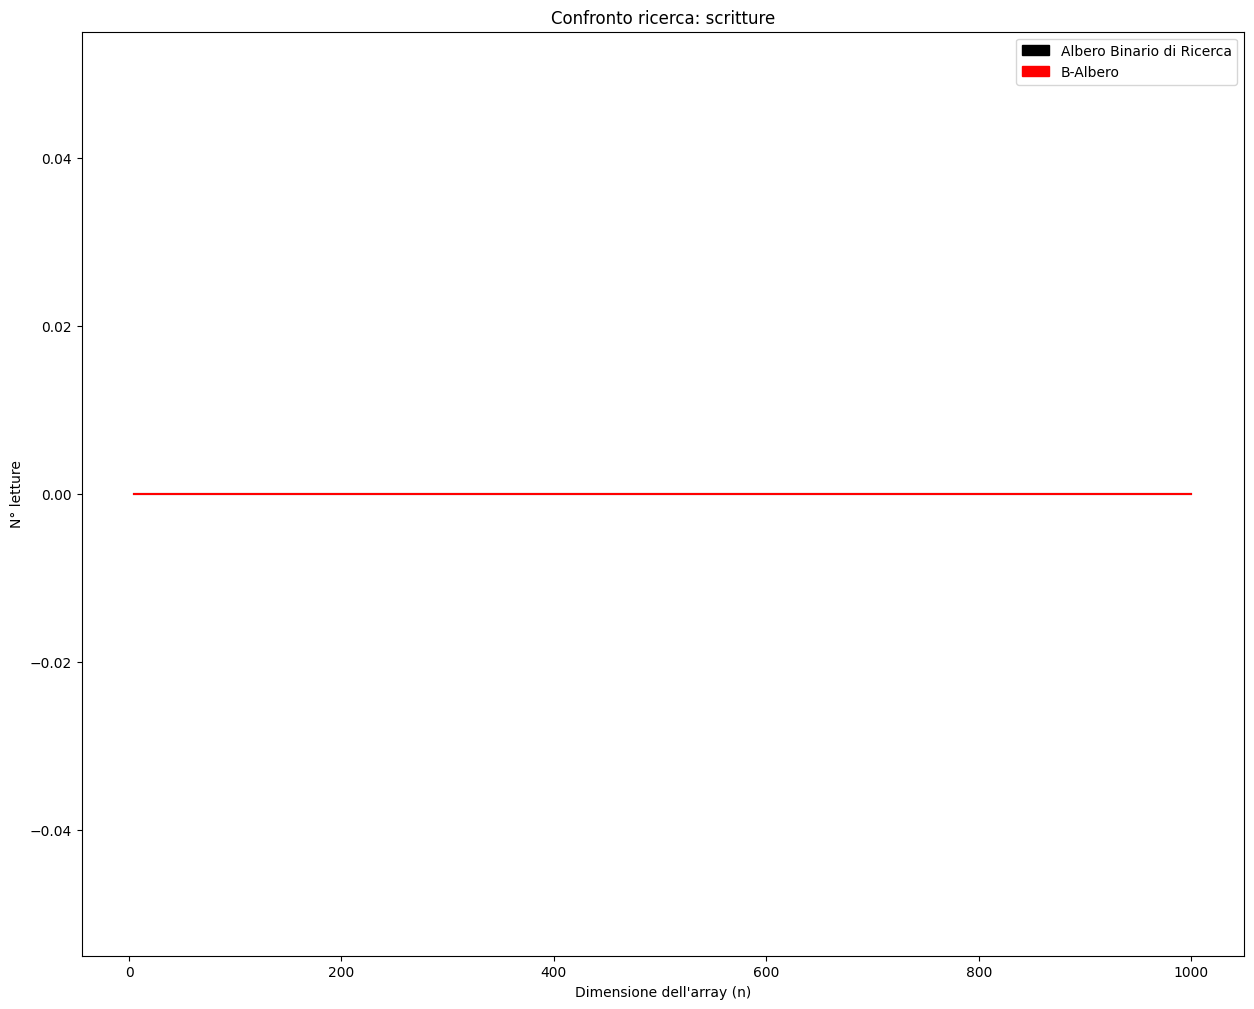
\includegraphics[width=\textwidth]{comparison-graphs/search-w-t250.png}
        \caption{Ricerca}
        \label{fig:compgraphsearchwrite250}
    \end{subfigure}
    \caption{Grafici di confronto delle scritture con $t=250$}
    \label{fig:compgraphread250}
\end{figure}


\subsubsection{Alberi a confronto nel numero di letture e scritture con $t = 1000$}

\begin{comment}
\begin{figure}[H]
    \centering
    \begin{subfigure}[b]{0.49\textwidth}
        \centering
        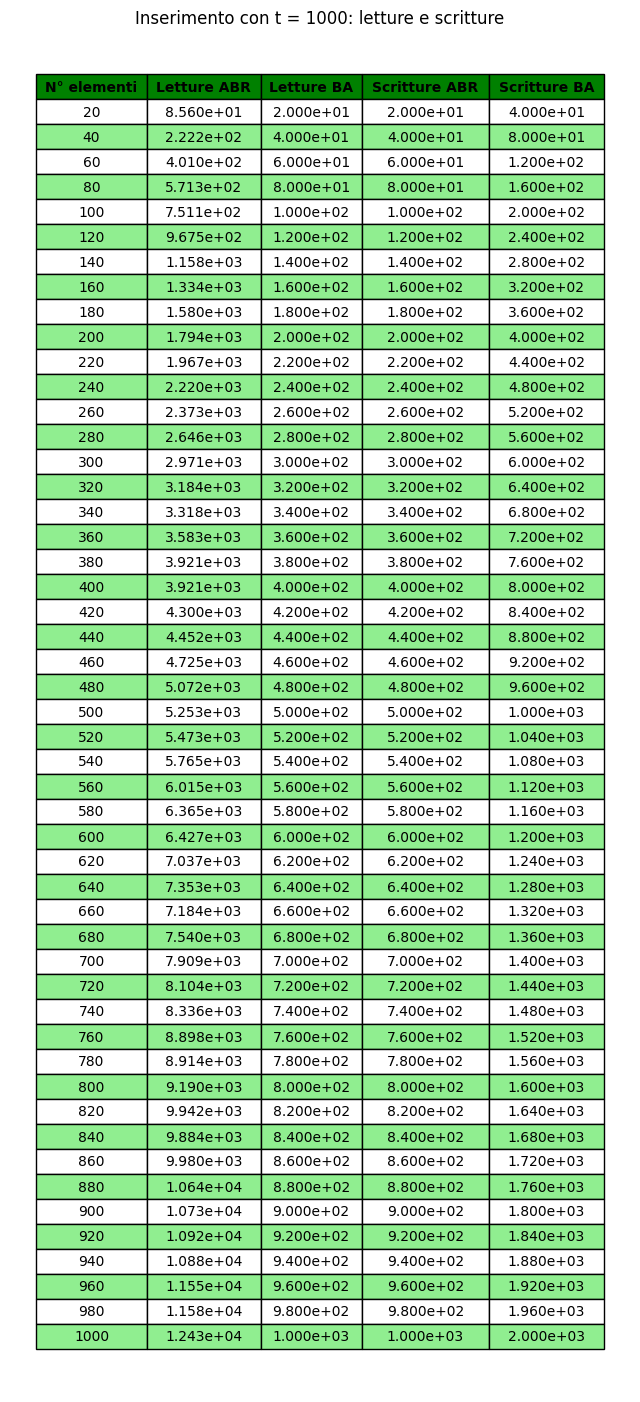
\includegraphics[width=\textwidth]{tables/insert-wr-t1000.png}
        \caption{Inserimento, letture e scritture}
        \label{fig:tableinsertwr1000}
    \end{subfigure}
    \hfill
    \begin{subfigure}[b]{0.49\textwidth}
        \centering
        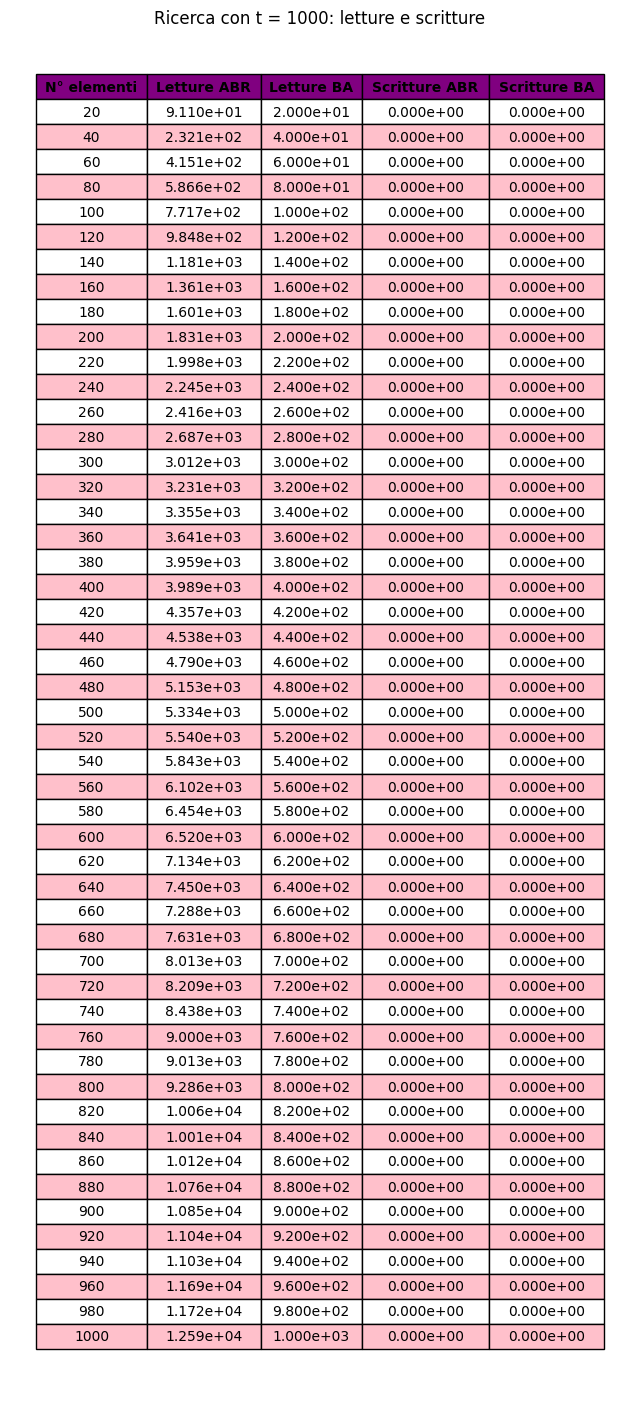
\includegraphics[width=\textwidth]{tables/search-wr-t1000.png}
        \caption{Ricerca, letture e scritture}
        \label{fig:tablesearchwr1000}
    \end{subfigure}
    \caption{Tabelle scritture e letture con $t=1000$}
    \label{fig:tablewr1000}
\end{figure}
\end{comment}

\begin{figure}[H]
    \centering
    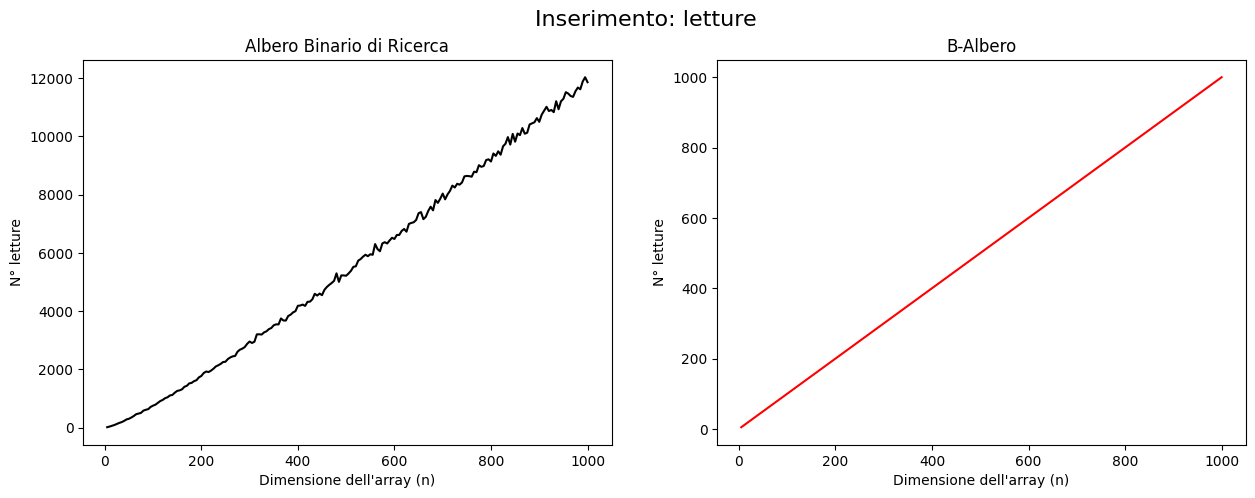
\includegraphics[width=\textwidth]{side-graphs/insert-r-t1000.png}
    \caption{Grafico delle letture dell'Inserimento con $t=1000$}
    \label{fig:sidegraphinsertread1000}
\end{figure}
    
\begin{figure}[H]
    \centering
    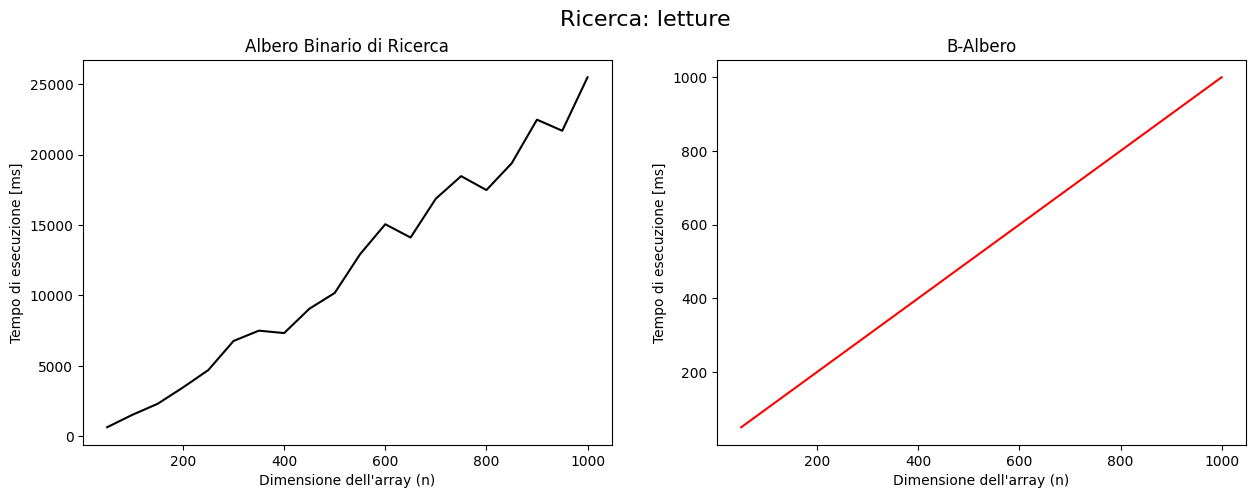
\includegraphics[width=\textwidth]{side-graphs/search-r-t1000.png}
    \caption{Grafico delle letture della Ricerca con $t=1000$}
    \label{fig:sidegraphsearchread1000}
\end{figure}

\begin{figure}[H]
    \centering
    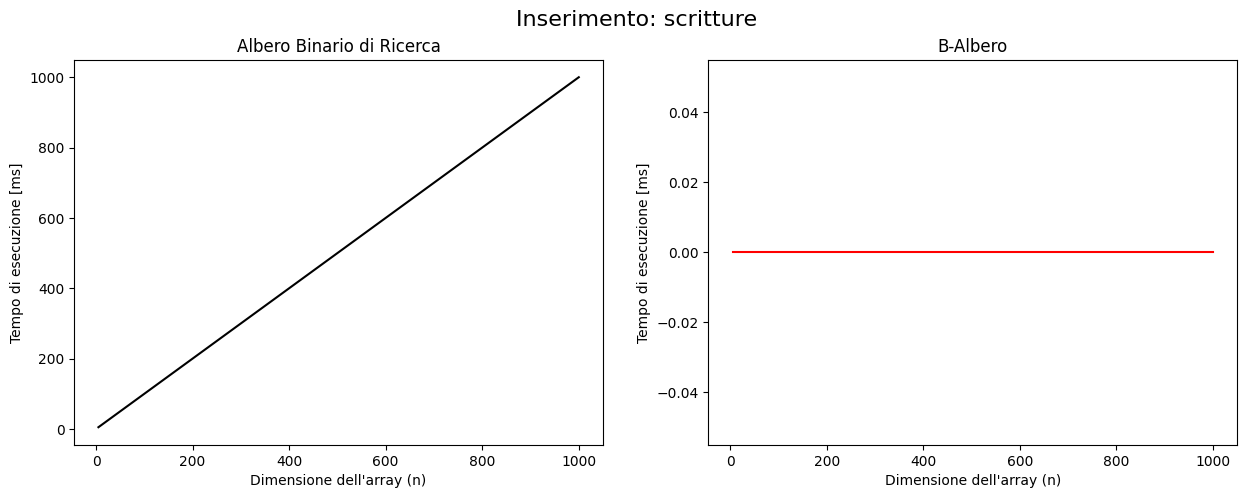
\includegraphics[width=\textwidth]{side-graphs/insert-w-t1000.png}
    \caption{Grafico delle scritture dell'Inserimento con $t=1000$}
    \label{fig:sidegraphinsertwrite1000}
\end{figure}
    
\begin{figure}[H]
    \centering
    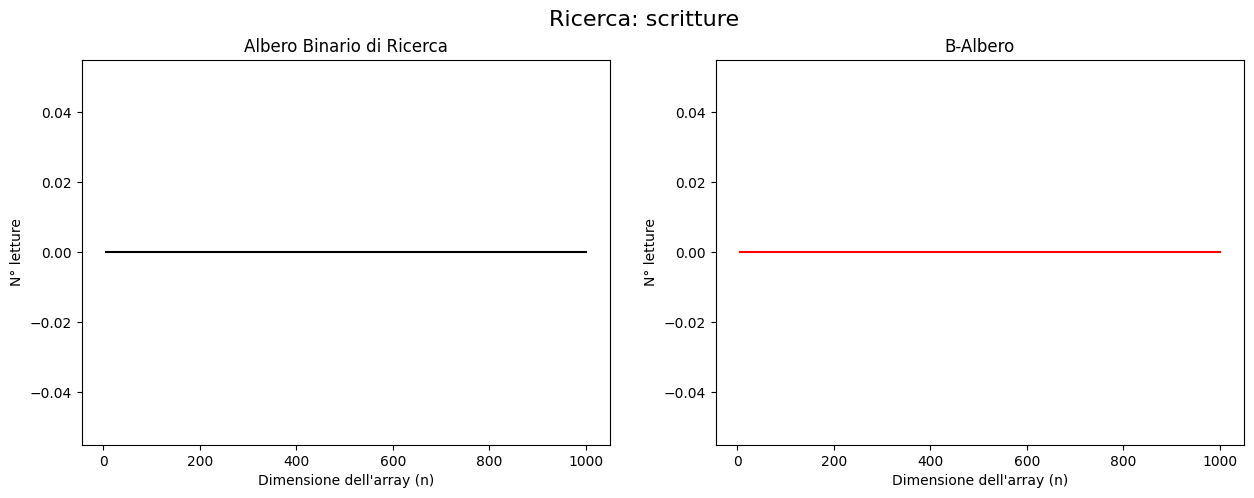
\includegraphics[width=\textwidth]{side-graphs/search-w-t1000.png}
    \caption{Grafico delle scritture della Ricerca con $t=1000$}
    \label{fig:sidegraphsearchwrite1000}
\end{figure}

\begin{figure}[H]
    \centering
    \begin{subfigure}[b]{0.49\textwidth}
        \centering
        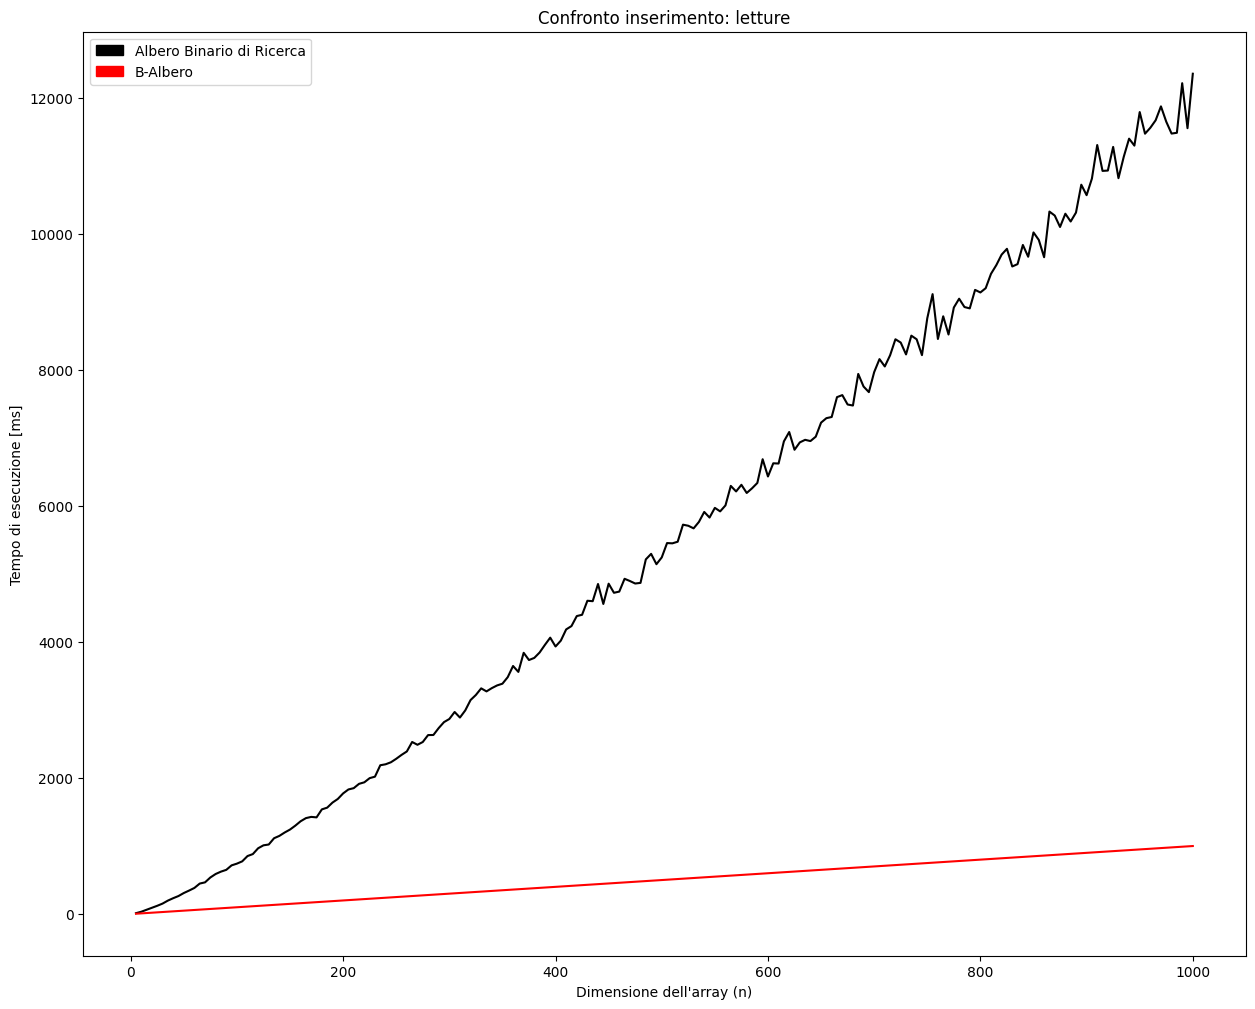
\includegraphics[width=\textwidth]{comparison-graphs/insert-r-t1000.png}
        \caption{Inserimento}
        \label{fig:compgraphinsertread1000}
    \end{subfigure}
    \hfill
    \begin{subfigure}[b]{0.49\textwidth}
        \centering
        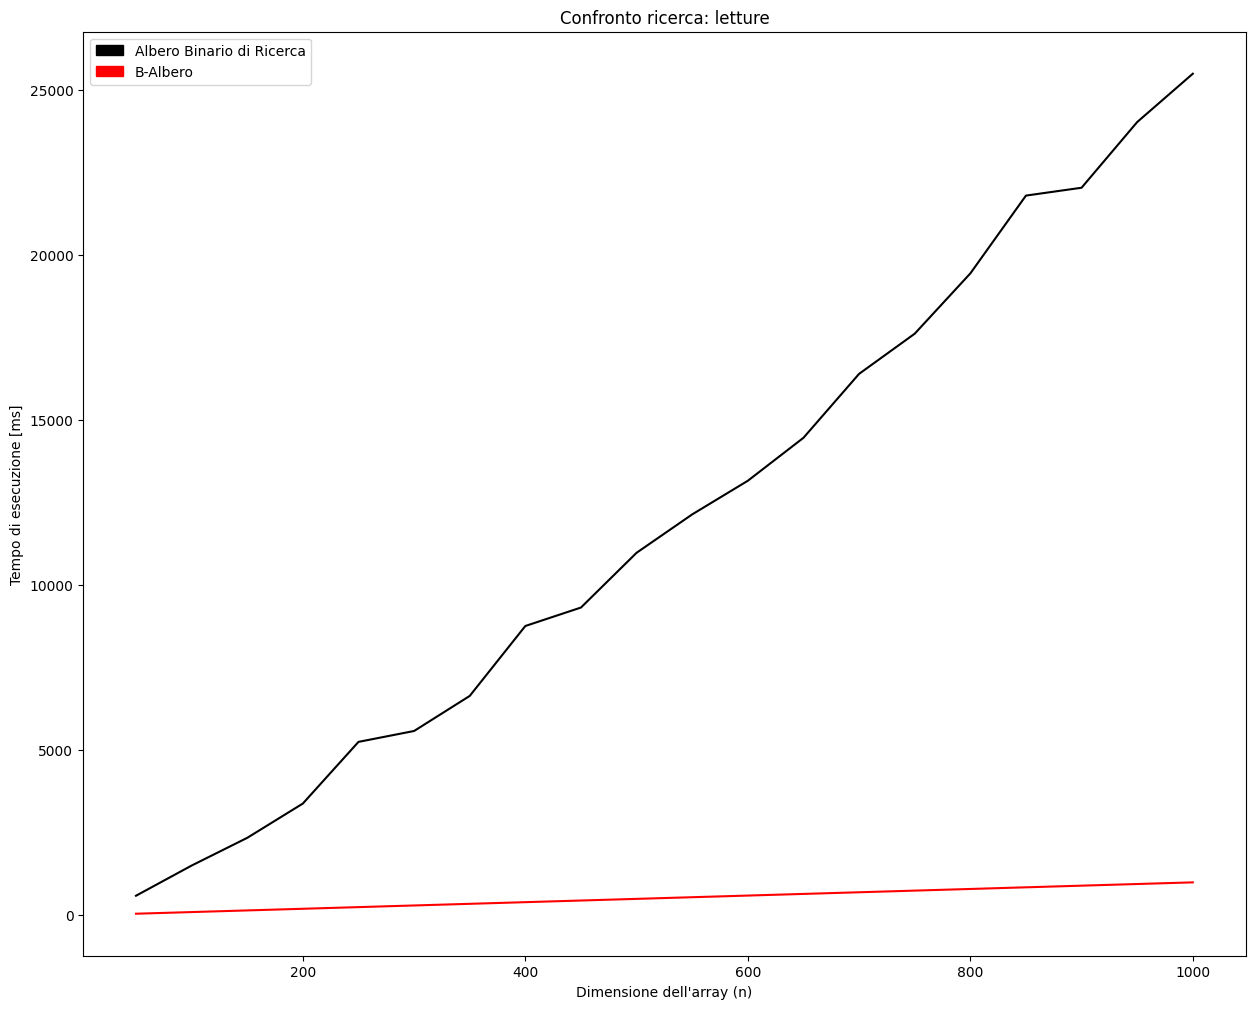
\includegraphics[width=\textwidth]{comparison-graphs/search-r-t1000.png}
        \caption{Ricerca}
        \label{fig:compgraphsearchread1000}
    \end{subfigure}
    \caption{Grafici di confronto delle letture con $t=1000$}
    \label{fig:compgraphread1000}
\end{figure}

\begin{figure}[H]
    \centering
    \begin{subfigure}[b]{0.49\textwidth}
        \centering
        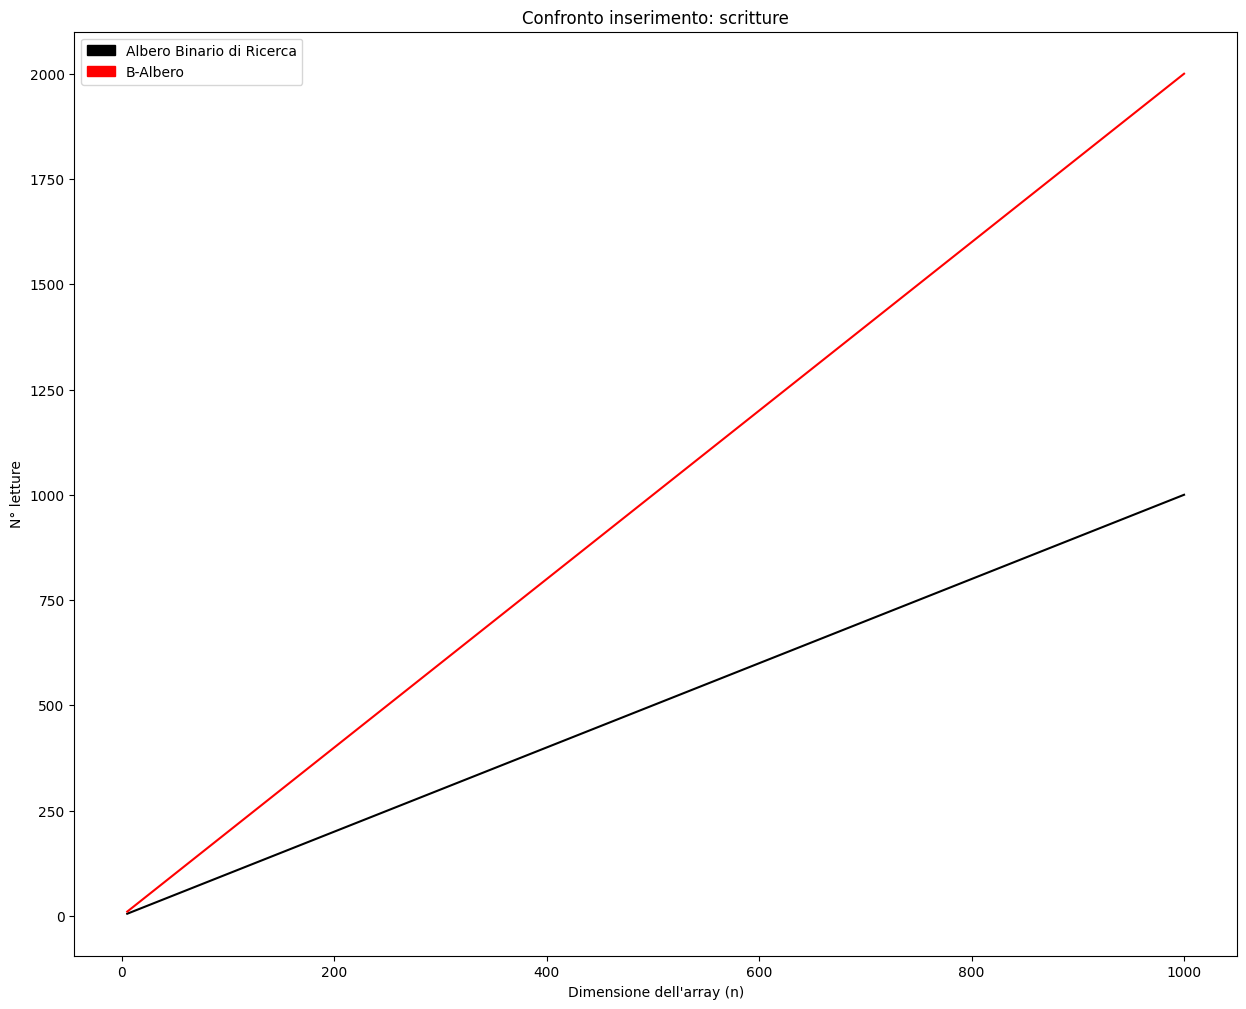
\includegraphics[width=\textwidth]{comparison-graphs/insert-w-t1000.png}
        \caption{Inserimento}
        \label{fig:compgraphinsertwrite1000}
    \end{subfigure}
    \hfill
    \begin{subfigure}[b]{0.49\textwidth}
        \centering
        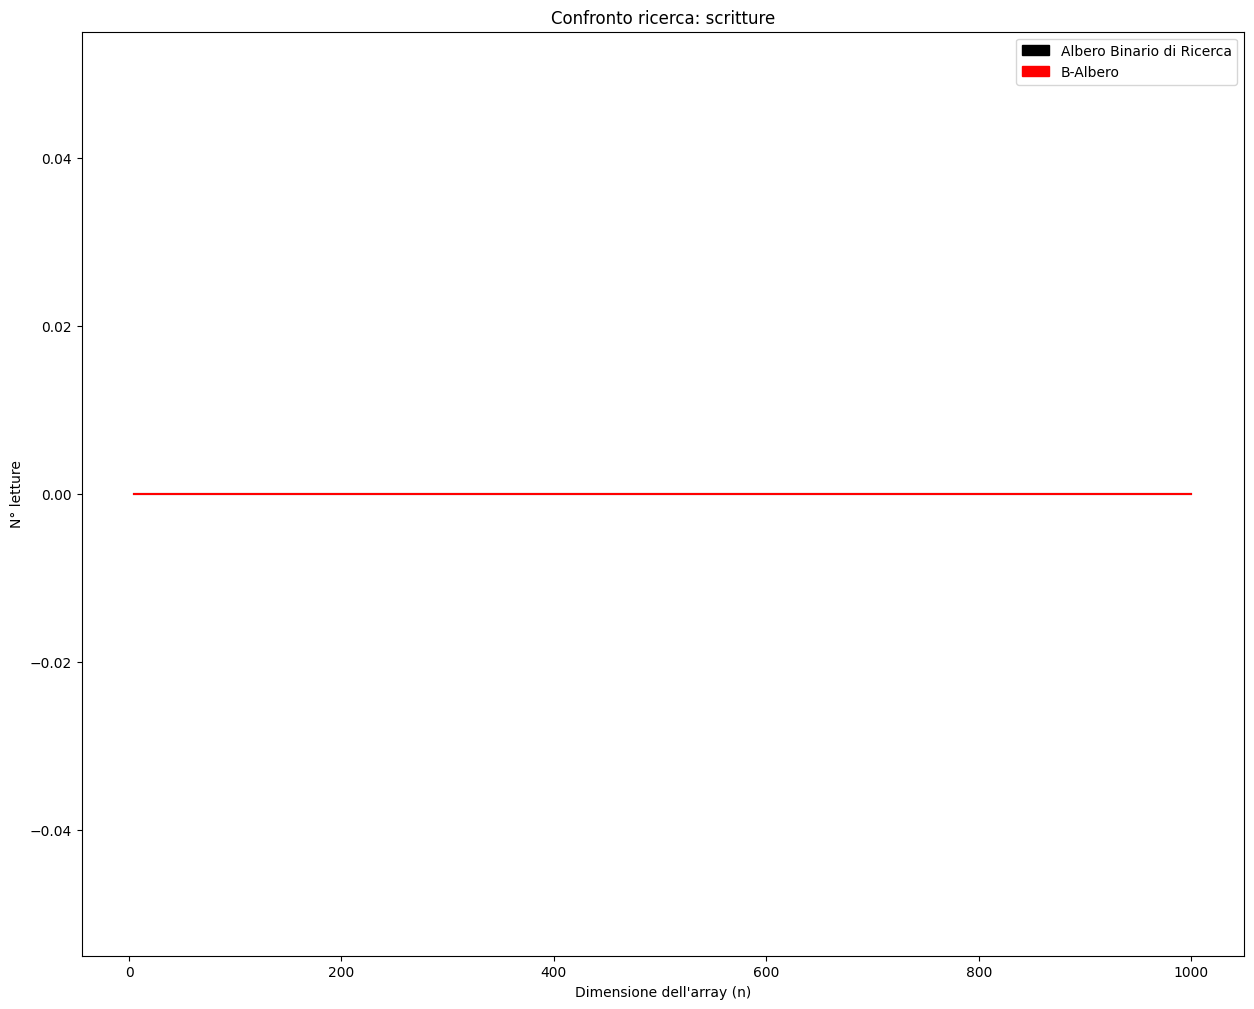
\includegraphics[width=\textwidth]{comparison-graphs/search-w-t1000.png}
        \caption{Ricerca}
        \label{fig:compgraphsearchwrite1000}
    \end{subfigure}
    \caption{Grafici di confronto delle scritture con $t=1000$}
    \label{fig:compgraphread1000}
\end{figure}



\subsection{Tesi e sintesi finale}
\label{TesiSintesiFinale_1}
Possiamo dare le seguenti conclusioni:
\begin{itemize}
    \item Complessità degli algoritmi:\\
        I metodi di inserimento e ricerca nei B-alberi hanno una complessità asintotica ottimale di $O(h) = O(\log_t n)$, dove $n$ è il numero di nodi nell'albero. Questa complessità è mantenuta anche nel caso peggiore, garantendo prestazioni efficienti.
    \item Tempo di esecuzione:\\
        Nel caso di un inserimento e la ricerca in catena nei B-alberi mantengono una complessità temporale ottimale di $O(log_t n * nTests)$, simile agli alberi ABR. Tuttavia, nei casi più complessi, la complessità è notevolmente migliorata rispetto agli ABR, mantenendo tempi di esecuzione più bassi.
    
    \item Influenza del riequilibrio:\\
        Nei B-alberi, il riequilibrio è intrinseco al processo di inserimento e non richiede passi aggiuntivi come negli ABR. Questo contribuisce a tempi di esecuzione più consistenti e prevedibili per l'inserimento e la ricerca, indipendentemente dal tipo di input.
    
    \item Variazione dei tempi con range di chiavi:\\
        Nel caso di operazioni casuali, i B-alberi possono mantenere tempi di esecuzione stabili anche con variazioni nel range delle chiavi. La struttura bilanciata dei B-alberi riduce l'impatto della distribuzione delle chiavi sull'efficienza delle operazioni.
    
    \item Conclusioni generali:\\
        I B-alberi dimostrano una robusta efficienza nelle operazioni di inserimento e ricerca, con una complessità che scala in modo ottimale con l'aumentare della dimensione dell'albero. Il riequilibrio automatico contribuisce a mantenere prestazioni stabili e prevedibili in una varietà di scenari, rendendo i B-alberi una scelta affidabile per applicazioni che richiedono una gestione efficiente di grandi quantità di dati.

\end{itemize}



